Now to discuss a possible shared key (symmetric key) algorithm that could be used as Enc$_\lambda$ in GCM.
\begin{Def}[Advanced Encryption Standard (AES)]

    \label{theo:aes}
    During a worldwide competition in 2001, the National Institute of Standards and Technology (NIST) selected the Rijndael algorithm as the Advanced Encryption Standard (AES).
    AES is a symmetric key block cipher that encrypts plaintext (PT) in 128-bit blocks. AES works in rounds permuting the PT with partial keys generated from the initial key.
    \begin{itemize}
        \item \textbf{Key Expansion}: An initial key is expanded into a key schedule. These keys will be assigned to each round. 
        The rounds needed depend on the initial key size:
        \begin{enumerate}
            \item 128-bit key: 10 rounds, 11 keys.
            \item 192-bit key: 12 rounds, 13 keys.
            \item 256-bit key: 14 rounds, 15 keys.
        \end{enumerate}
        \item \textbf{Input Transformation}: The PT is transformed into a $4\times4$ matrix, called the \textbf{State}. The 
        state undergoes four main operations per round:
        \begin{enumerate}
            \item \textbf{SubBytes}: Each byte is substituted with a value from the S-Box.
            \item \textbf{ShiftRows}: Each row is shifted left by an offset.
            \item \textbf{MixColumns}: Each column is mixed with a fixed matrix.
            \item \textbf{AddRoundKey}: Each byte in the State is XORed with a sub-key. \hfill \cite{satish2024aes} \cite{nist_aes2001} \cite{brainkartAES2018}
        \end{enumerate}
    \end{itemize}

    
\end{Def}

\newpage 

\begin{Def}[Key Expansion]
    
        \label{theo:key_expansion}
        Key expansion, an AES process which takes a single key and expands it into multiple keys. The initial key 
        is broken up into 16-byte $4\times4$ matrices. Each column a \textbf{Word} (32-bits). The process follows 
        four main steps:
        \begin{center}
            \textbf{RotWord}$\rightarrow$\textbf{SubWord}$\rightarrow$\textbf{Rcon}$\rightarrow$\textbf{XOR}.\\
            (Rotate Word, Substitute Word, Round Constant, XOR)
        \end{center}
        
        \noindent
        This generates a \textbf{Sub-Key} for one round. Each round generates for the next round.
\end{Def}

\noindent
\textbf{AES Key Expansion:} Given the an initial 128-bit key, $\lambda_0$ ``my\_secret\_key001'':\\

\vspace{1em}

\hspace{-3em}
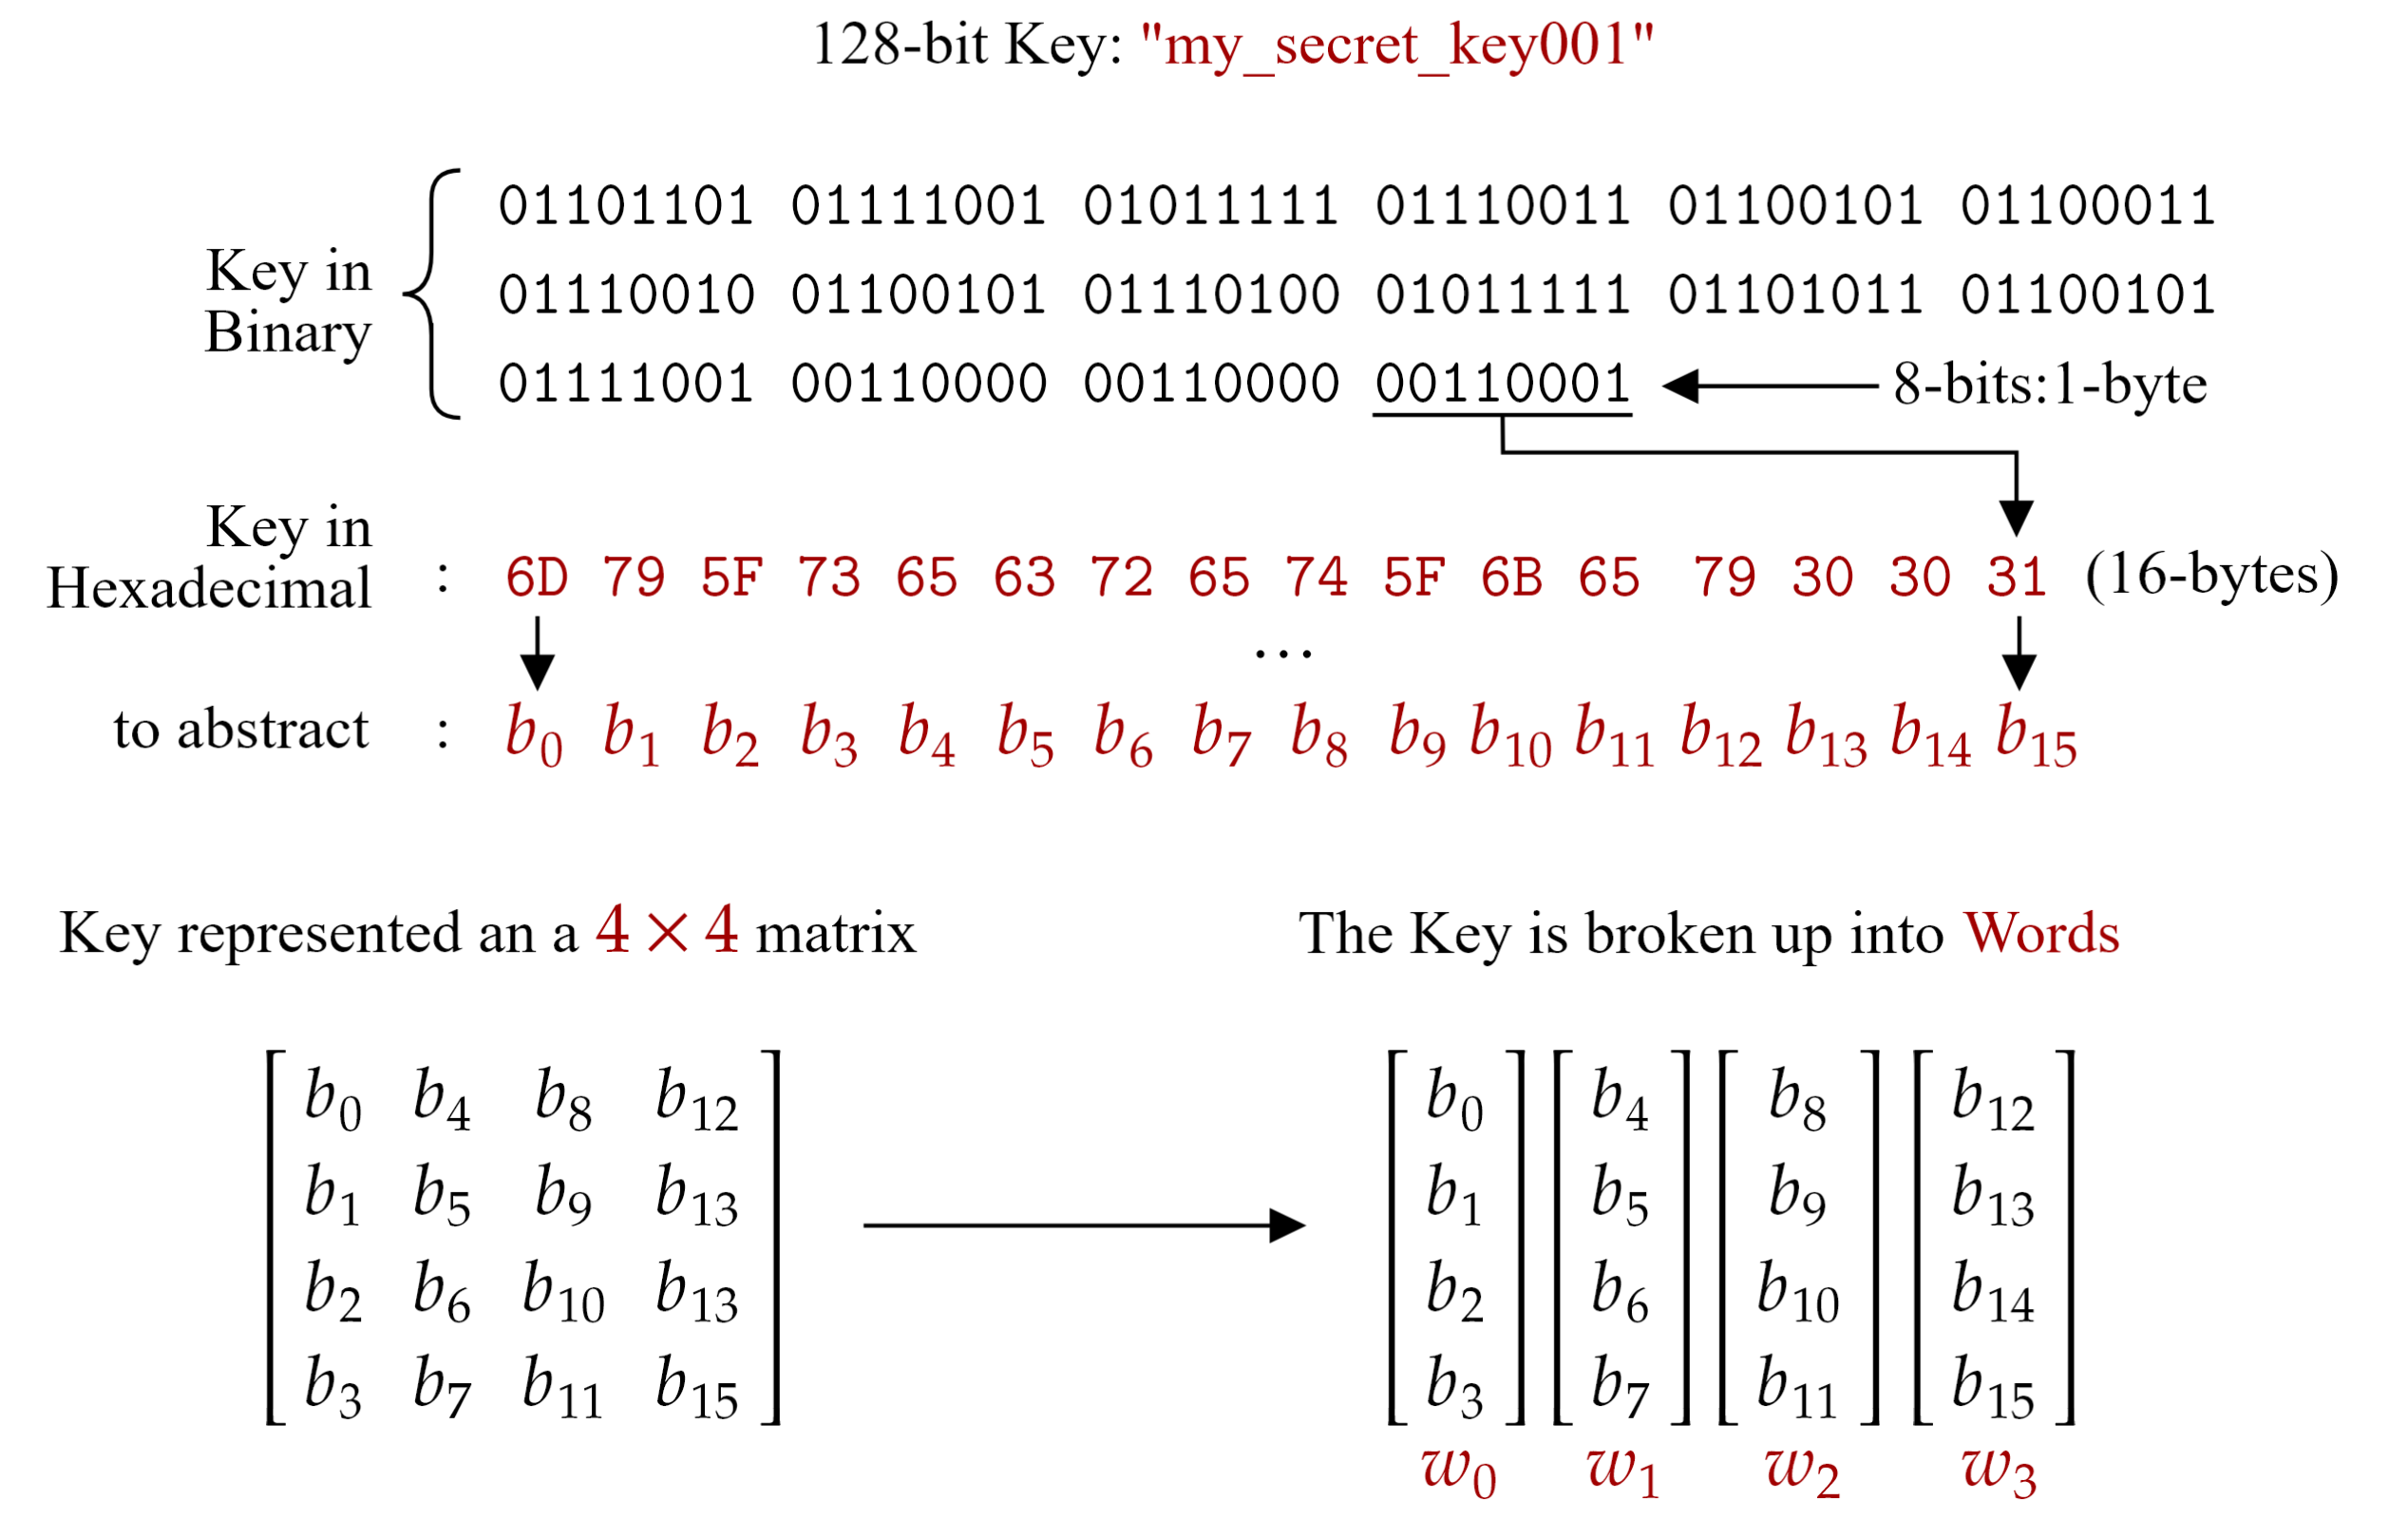
\includegraphics [width=1.1\textwidth]{Sections/sec/enc/aes/input.png}

\vspace{3em}
\noindent
These Words $w_0, w_1, w_2, w_3$ are the initial key. This will then generate the rest of the Words needed.
This first group is the first sub-key $s_0$ for the first round.

\newpage 

\hspace{-3em}
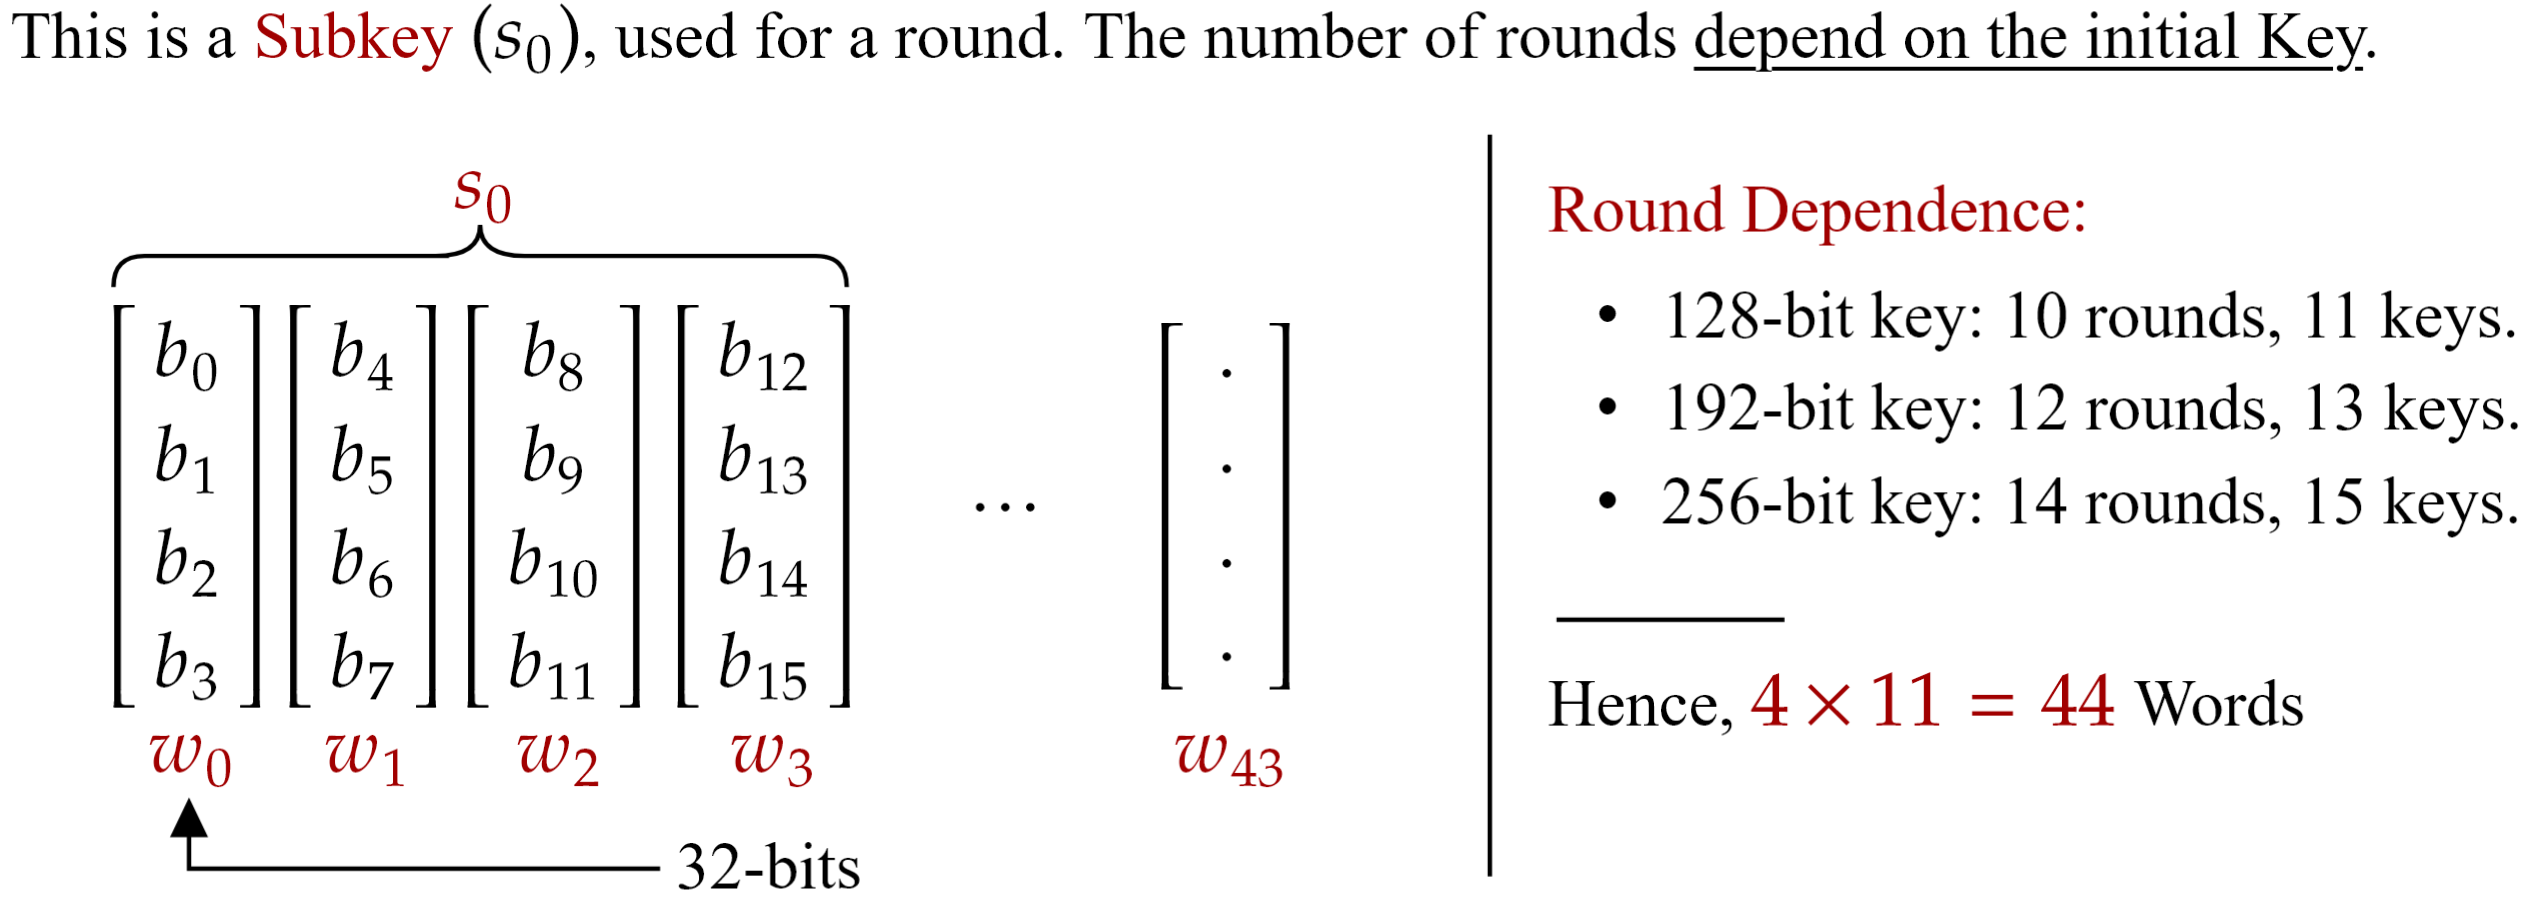
\includegraphics[width=1.1\textwidth]{Sections/sec/enc/aes/subkey.png}

\vspace{1em}
\noindent
\textcolor{gray}{Rounds depend on $\|\lambda_0\|$: 128-bits $\rightarrow$ 10 rounds, 192-bits $\rightarrow$ 12 rounds, 256-bits $\rightarrow$ 14 rounds.}

\vspace{1em}
\hspace{-3em}
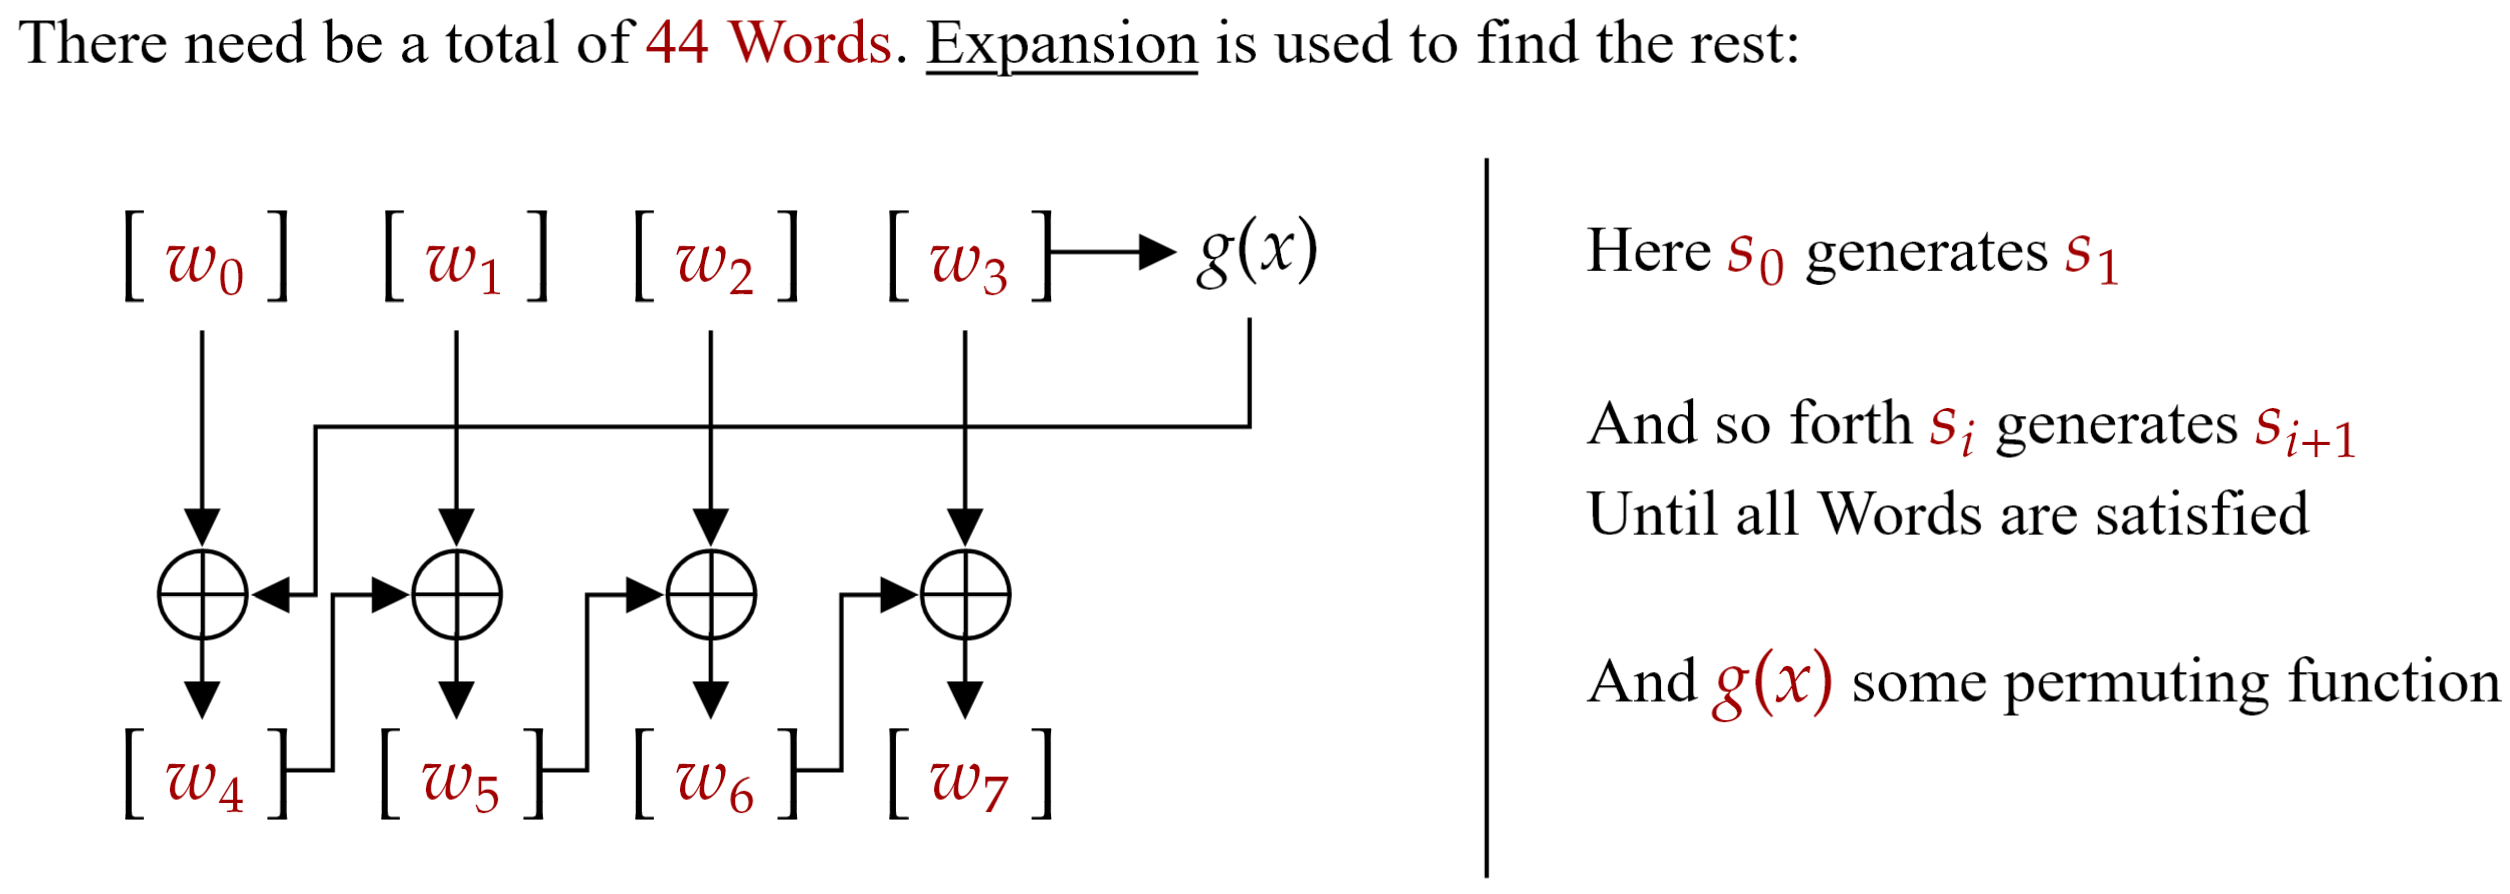
\includegraphics[width=1.1\textwidth]{Sections/sec/enc/aes/round_gen.png}

\noindent
\textcolor{gray}{The $g(x):=RotWord \circ SubWord \circ Rcon \circ XOR$, generating the next sub-key $s_1$.}

\vspace{1em}
\hspace{-3em}
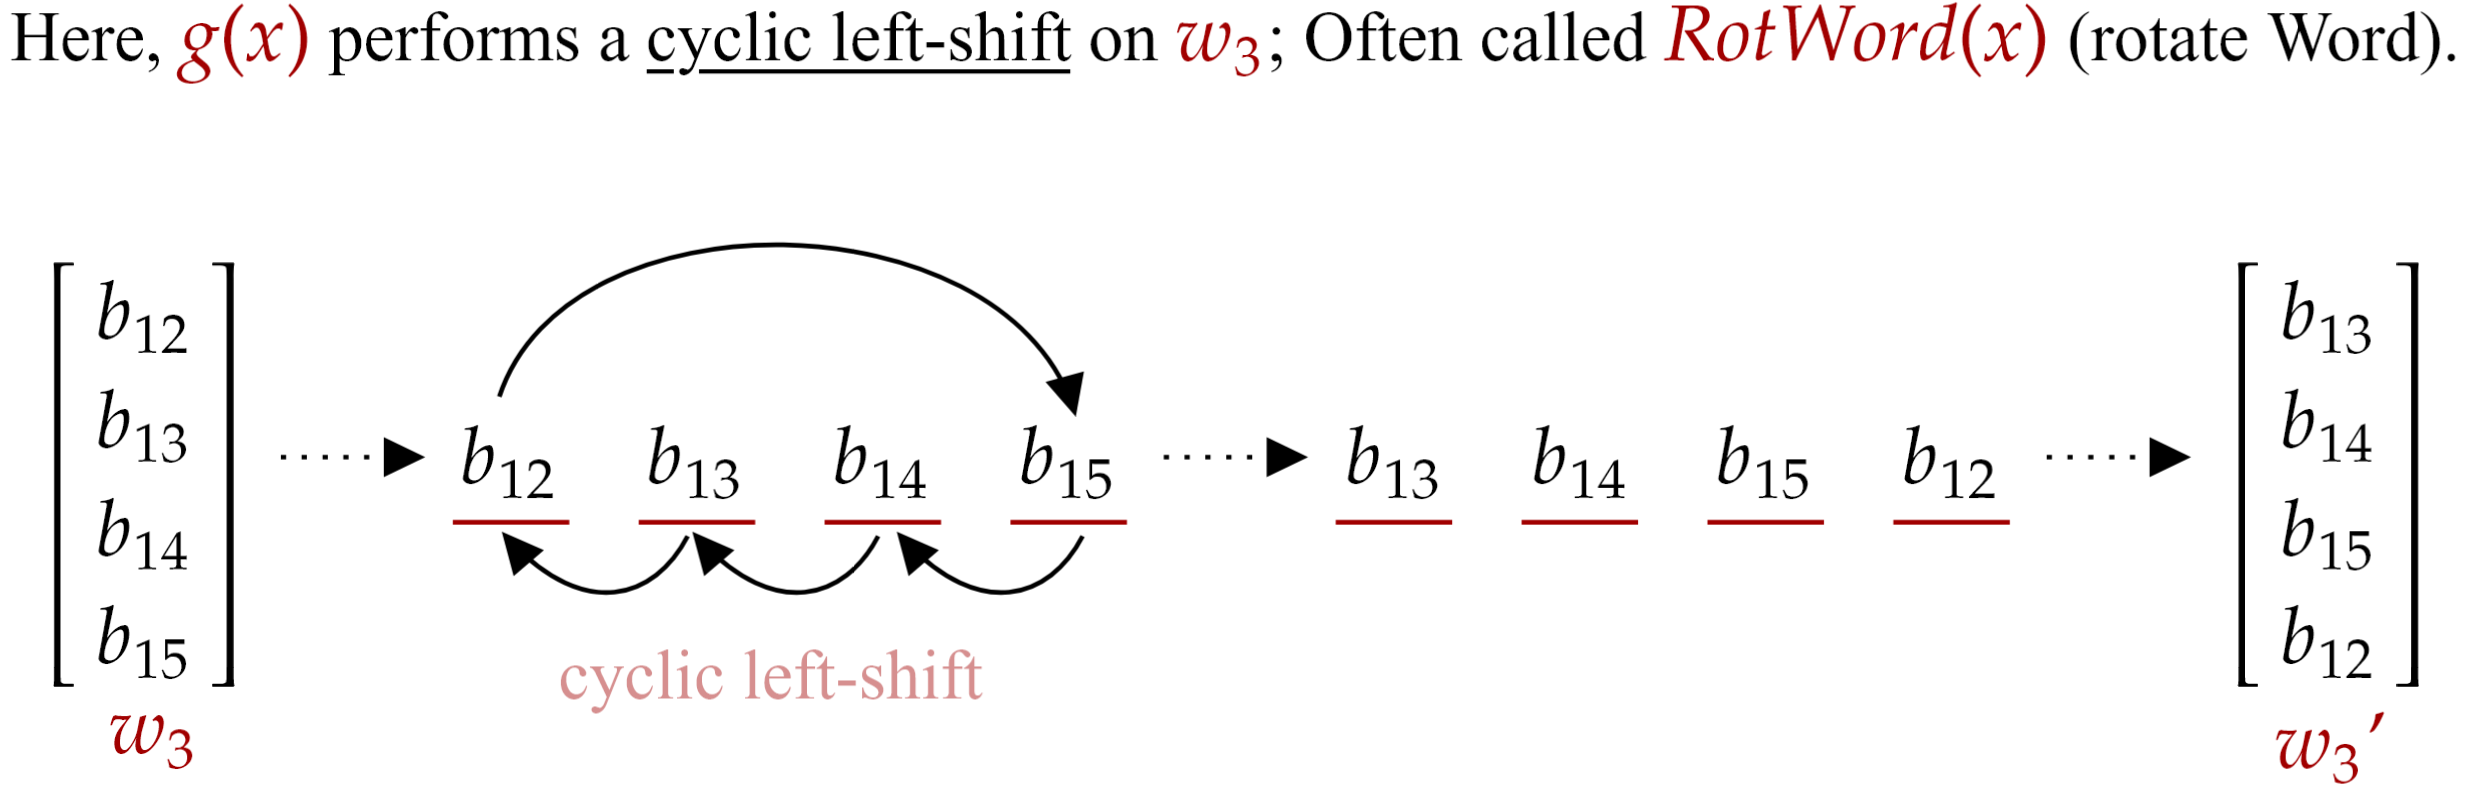
\includegraphics[width=1.1\textwidth]{Sections/sec/enc/aes/g_func.png}

\newpage
\noindent
\begin{Def}[Nibble]

    \label{theo:nibble}
    A \textbf{nibble} is a four-bit aggregation, referring to ``half a \textbf{byte}.'' A nibble splits 8-bits into two 4-bit values,
    the \textbf{upper nibble} and the \textbf{lower nibble}. E.g., given the hex value $0A$,
    the upper and lower nibble is $0$ and $A$ respectively.
\end{Def}
Now to quickly introduce some concepts needed for the AES borrowed from group theory.
\begin{Def}[Field]

    \label{def:field}
    A \textbf{field} is a set of elements equipped with two operations, addition and multiplication, such that the following properties hold:
    \begin{itemize}
        \item \textbf{Closure}: Adding or multiplying any two elements in the set remains in the set.
        \item \textbf{Associativity}: Addition and multiplication are associative.
        \item \textbf{Commutativity}: Addition and multiplication are commutative.
        \item \textbf{Identities}: There exist identity elements for addition (0) and multiplication (1).
        \item \textbf{Inverses}: Every element has an additive inverse (negative) and, except for 0, a multiplicative inverse (reciprocal).
        \item \textbf{Distributivity}: Multiplication distributes over addition.
    \end{itemize}

    \noindent
    E.g., The set of real numbers $\mathbb{R}$, with standard addition and multiplication, forms a field.
\end{Def}
\begin{theo}[Abel Ruffini Theorem]

    \label{theo:abel_ruffini}
    There is no general for solving polynomials of degree five or higher. Moreover,
    no formula is possible using these finite amount of: $+,-,\times,\div,\sqrt[n]{x}$.
\end{theo}

\noindent
This will play a key part in the AES algorithm, stopping attackers from reversing the encryption process.

\newpage

\begin{Def}[Galois Field $GF(2^8)$]

    \label{def:galois_field}
    The Galois Field $GF(2^8)$ is a finite field consisting of $2^8 = 256$ elements, where each element is an 8-bit binary value (a byte).
    Addition and multiplication in $GF(2^8)$ are defined modulo an irreducible polynomial of degree 8 over $GF(2)$ (the binary field).
    
    \noindent
    In AES, the irreducible polynomial used is:
    \[
    p(x) = x^8 + x^4 + x^3 + x + 1.
    \]
\end{Def}

\vspace{-1em}
\begin{Tip}
    To learn more consider this video on Galois Theory: \href{https://www.youtube.com/watch?v=1EWUsef0iFs}{``Why is there no quintic formula?''}
\end{Tip}


\begin{Def}[AES S-Box]

    \label{theo:aes_sbox}
    The AES S-Box is a substitution box used in the AES algorithm. It is a $16\times16$ matrix of 8-bit values. 
    The first column and row represent the upper and lower nibble of the input byte. E.g., given $C7$, column $c0$ and row $07$ intersect $c6$.
\end{Def}
\[
\begin{array}{|>{\columncolor[gray]{0.8}}c|c|*{15}{c|}}
\hline
    \rowcolor{black} & \textcolor{white}{00} & \textcolor{white}{01} & \textcolor{white}{02} & \textcolor{white}{03} & \textcolor{white}{04} & \textcolor{white}{05} & \textcolor{white}{06} & \textcolor{white}{07} & \textcolor{white}{08} & \textcolor{white}{09} & \textcolor{white}{0a} & \textcolor{white}{0b} & \textcolor{white}{0c} & \textcolor{white}{0d} & \textcolor{white}{0e} & \textcolor{white}{0f} \\
\hline
00 & 63 & 7c & 77 & 7b & f2 & 6b & 6f & c5 & 30 & 01 & 67 & 2b & fe & d7 & ab & 76 \\
10 & ca & 82 & c9 & 7d & fa & 59 & 47 & f0 & ad & d4 & a2 & af & 9c & a4 & 72 & c0 \\
20 & b7 & fd & 93 & 26 & 36 & 3f & f7 & cc & 34 & a5 & e5 & f1 & 71 & d8 & 31 & 15 \\
30 & 04 & c7 & 23 & c3 & 18 & 96 & 05 & 9a & 07 & 12 & 80 & e2 & eb & 27 & b2 & 75 \\
40 & 09 & 83 & 2c & 1a & 1b & 6e & 5a & a0 & 52 & 3b & d6 & b3 & 29 & e3 & 2f & 84 \\
50 & 53 & d1 & 00 & ed & 20 & fc & b1 & 5b & 6a & cb & be & 39 & 4a & 4c & 58 & cf \\
60 & d0 & ef & aa & fb & 43 & 4d & 33 & 85 & 45 & f9 & 02 & 7f & 50 & 3c & 9f & a8 \\
70 & 51 & a3 & 40 & 8f & 92 & 9d & 38 & f5 & bc & b6 & da & 21 & 10 & ff & f3 & d2 \\
80 & cd & 0c & 13 & ec & 5f & 97 & 44 & 17 & c4 & a7 & 7e & 3d & 64 & 5d & 19 & 73 \\
90 & 60 & 81 & 4f & dc & 22 & 2a & 90 & 88 & 46 & ee & b8 & 14 & de & 5e & 0b & db \\
a0 & e0 & 32 & 3a & 0a & 49 & 06 & 24 & 5c & c2 & d3 & ac & 62 & 91 & 95 & e4 & 79 \\
b0 & e7 & c8 & 37 & 6d & d5 & 4e & a9 & 6c & 56 & f4 & ea & 65 & 7a & ae & 08 & ba \\
c0 & ba & 78 & 25 & 2e & 1c & a6 & b4 & c6 & e8 & dd & 74 & 1f & 4b & bd & 8b & 8a \\
d0 & 70 & 3e & b5 & 66 & 48 & 03 & f6 & 0e & 61 & 35 & 57 & 89 & 86 & c1 & 1d & 9e \\
e0 & e1 & f8 & 98 & 11 & 69 & d9 & 8e & 94 & 9b & 1e & 87 & e9 & ce & 55 & 28 & df \\
f0 & 8c & a1 & 89 & 0d & bf & e6 & 42 & 68 & 41 & 99 & 2d & 0f & b0 & 54 & bb & 16 \\
\hline
\end{array}
\]

\newpage 

\noindent
For reference, previous figures are shown again.

\begin{center}
    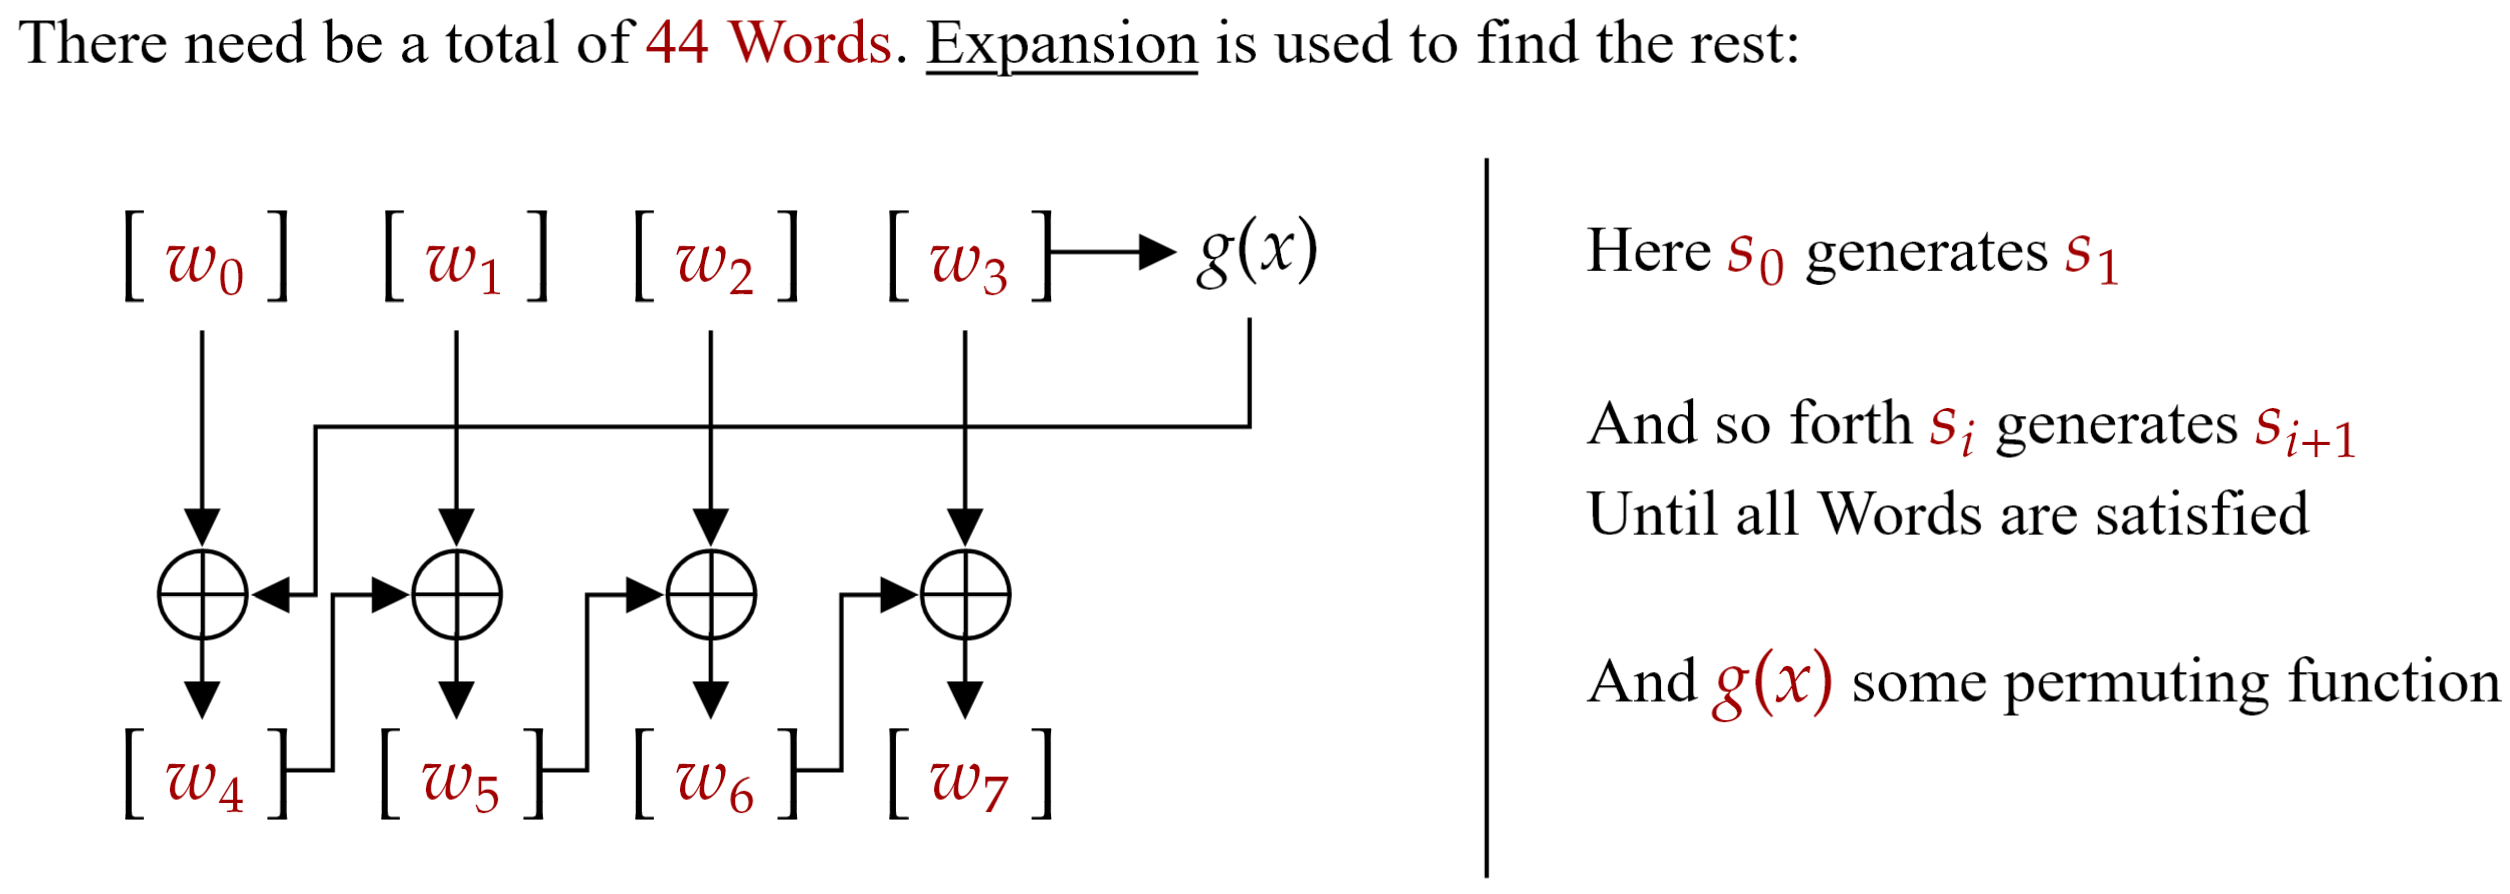
\includegraphics[width=.8\textwidth]{Sections/sec/enc/aes/round_gen.png}

    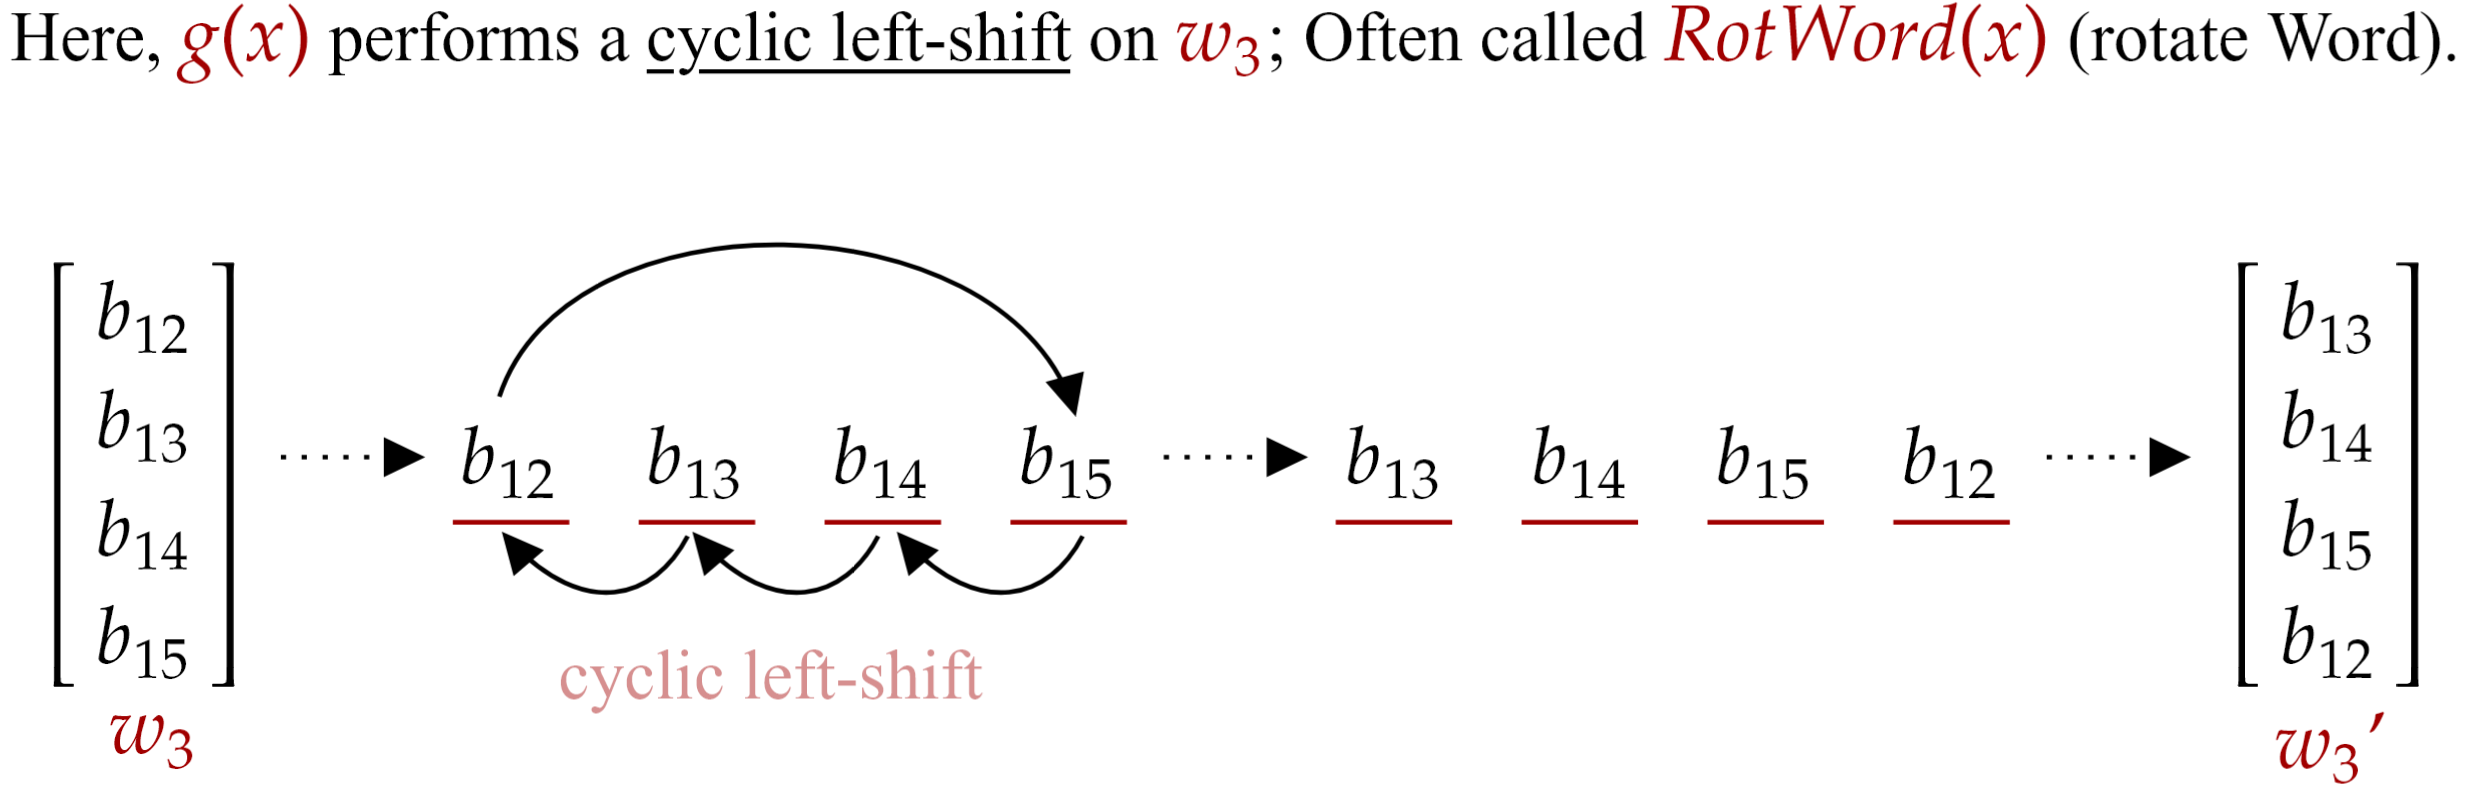
\includegraphics[width=.8\textwidth]{Sections/sec/enc/aes/g_func.png}

\end{center}

\vspace{1em}
\noindent

\hspace{-3em}
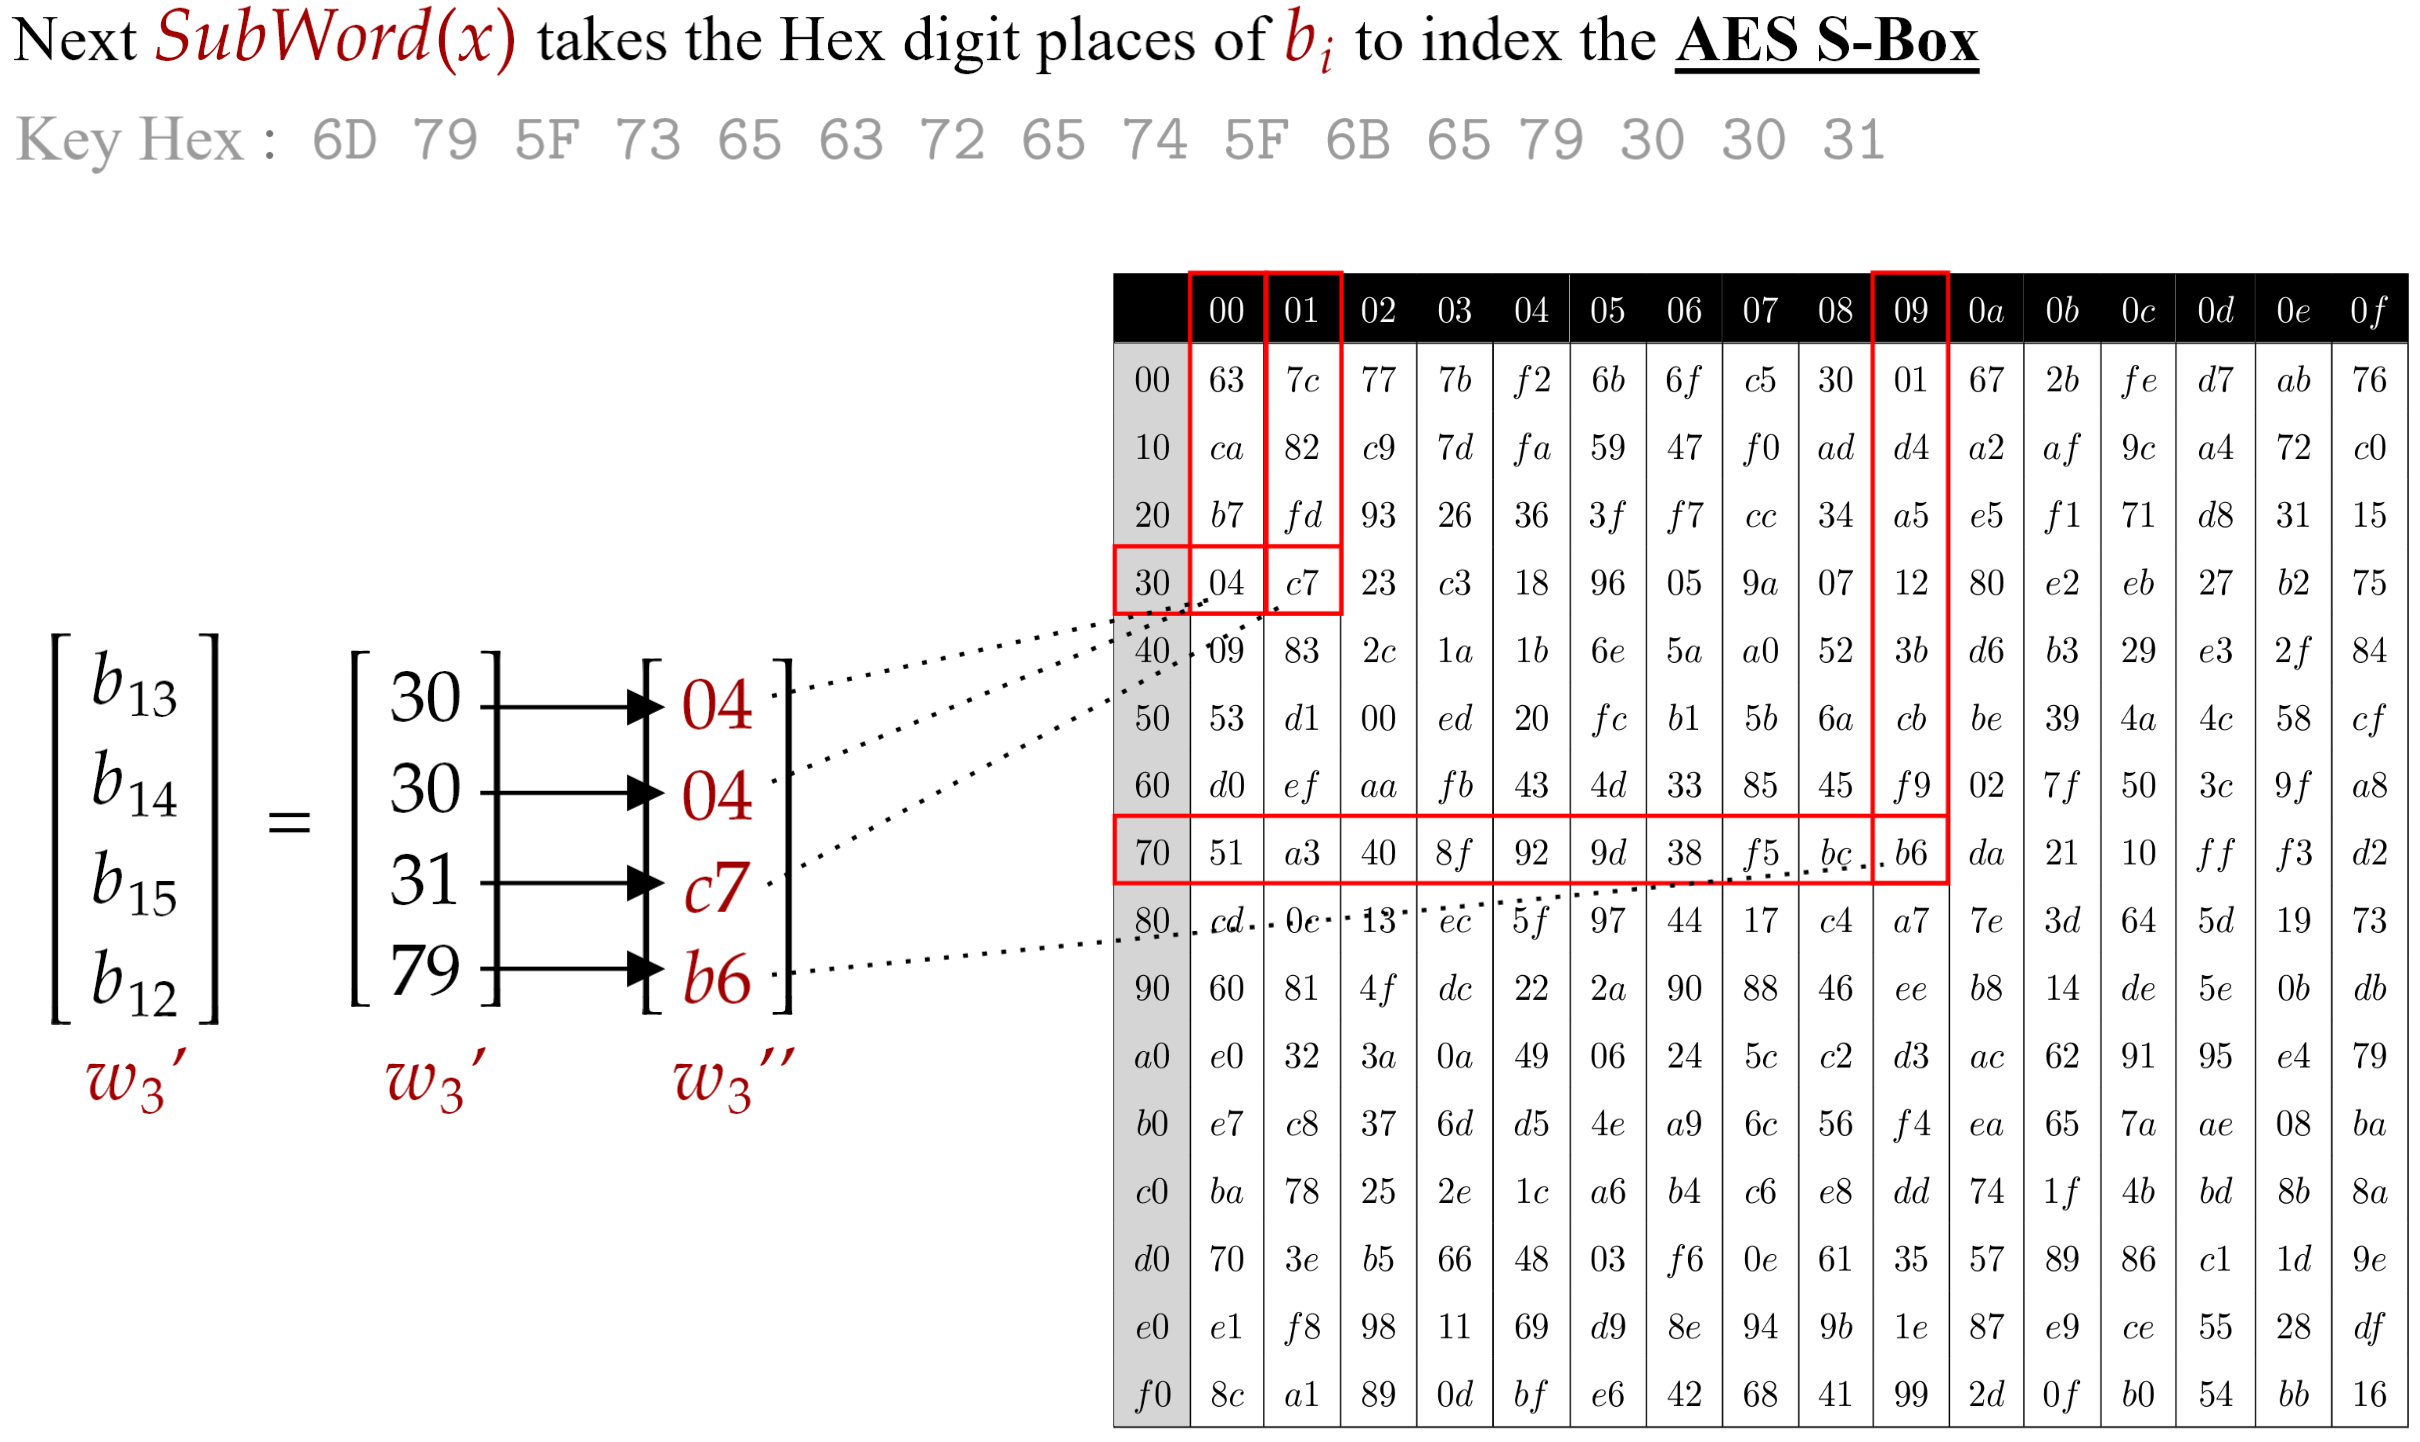
\includegraphics[width=1.1\textwidth]{Sections/sec/enc/aes/sub_word.png}

\newpage 

\begin{Def}[Round Constants]

    \label{theo:round_constants}
    Round constants take the output of $SubWord(x)$ and XOR the first byte with a constant value.
    The constant value, denoted $Rcon[j]$, is derived from powers of 2 in the Galois Field $GF(2^8)$, where the irreducible polynomial is $x^8 + x^4 + x^3 + x + 1$.

    Each round constant ensures the uniqueness of round keys during the AES key expansion process, introducing nonlinearity and breaking symmetry between rounds.
\end{Def}

\begin{table}[h!]
    \centering
    \renewcommand{\arraystretch}{1.4}
    \begin{tabular}{|c|c|c|}
    \hline
    \textbf{Round (i)} & \textbf{\textit{Rcon} Value} & \textbf{Power of 2 in GF(2\textsuperscript{8})} \\
    \hline
    1  & 0x01 00 00 00 & $2^0 = 1$     \\
    2  & 0x02 00 00 00 & $2^1 = 2$     \\
    3  & 0x04 00 00 00 & $2^2 = 4$     \\
    4  & 0x08 00 00 00 & $2^3 = 8$     \\
    5  & 0x10 00 00 00 & $2^4 = 16$    \\
    6  & 0x20 00 00 00 & $2^5 = 32$    \\
    7  & 0x40 00 00 00 & $2^6 = 64$    \\
    8  & 0x80 00 00 00 & $2^7 = 128$   \\
    9  & 0x1B 00 00 00 & $2^8 \, \text{mod poly}$ \\
    10 & 0x36 00 00 00 & $2^9 \, \text{mod poly}$ \\
    \hline
    \end{tabular}
    \caption{Round Constants, where poly:= $x^8 + x^4 + x^3 + x + 1$.}
    \label{tab:rcon-values}
\end{table}


\hspace{-3em}
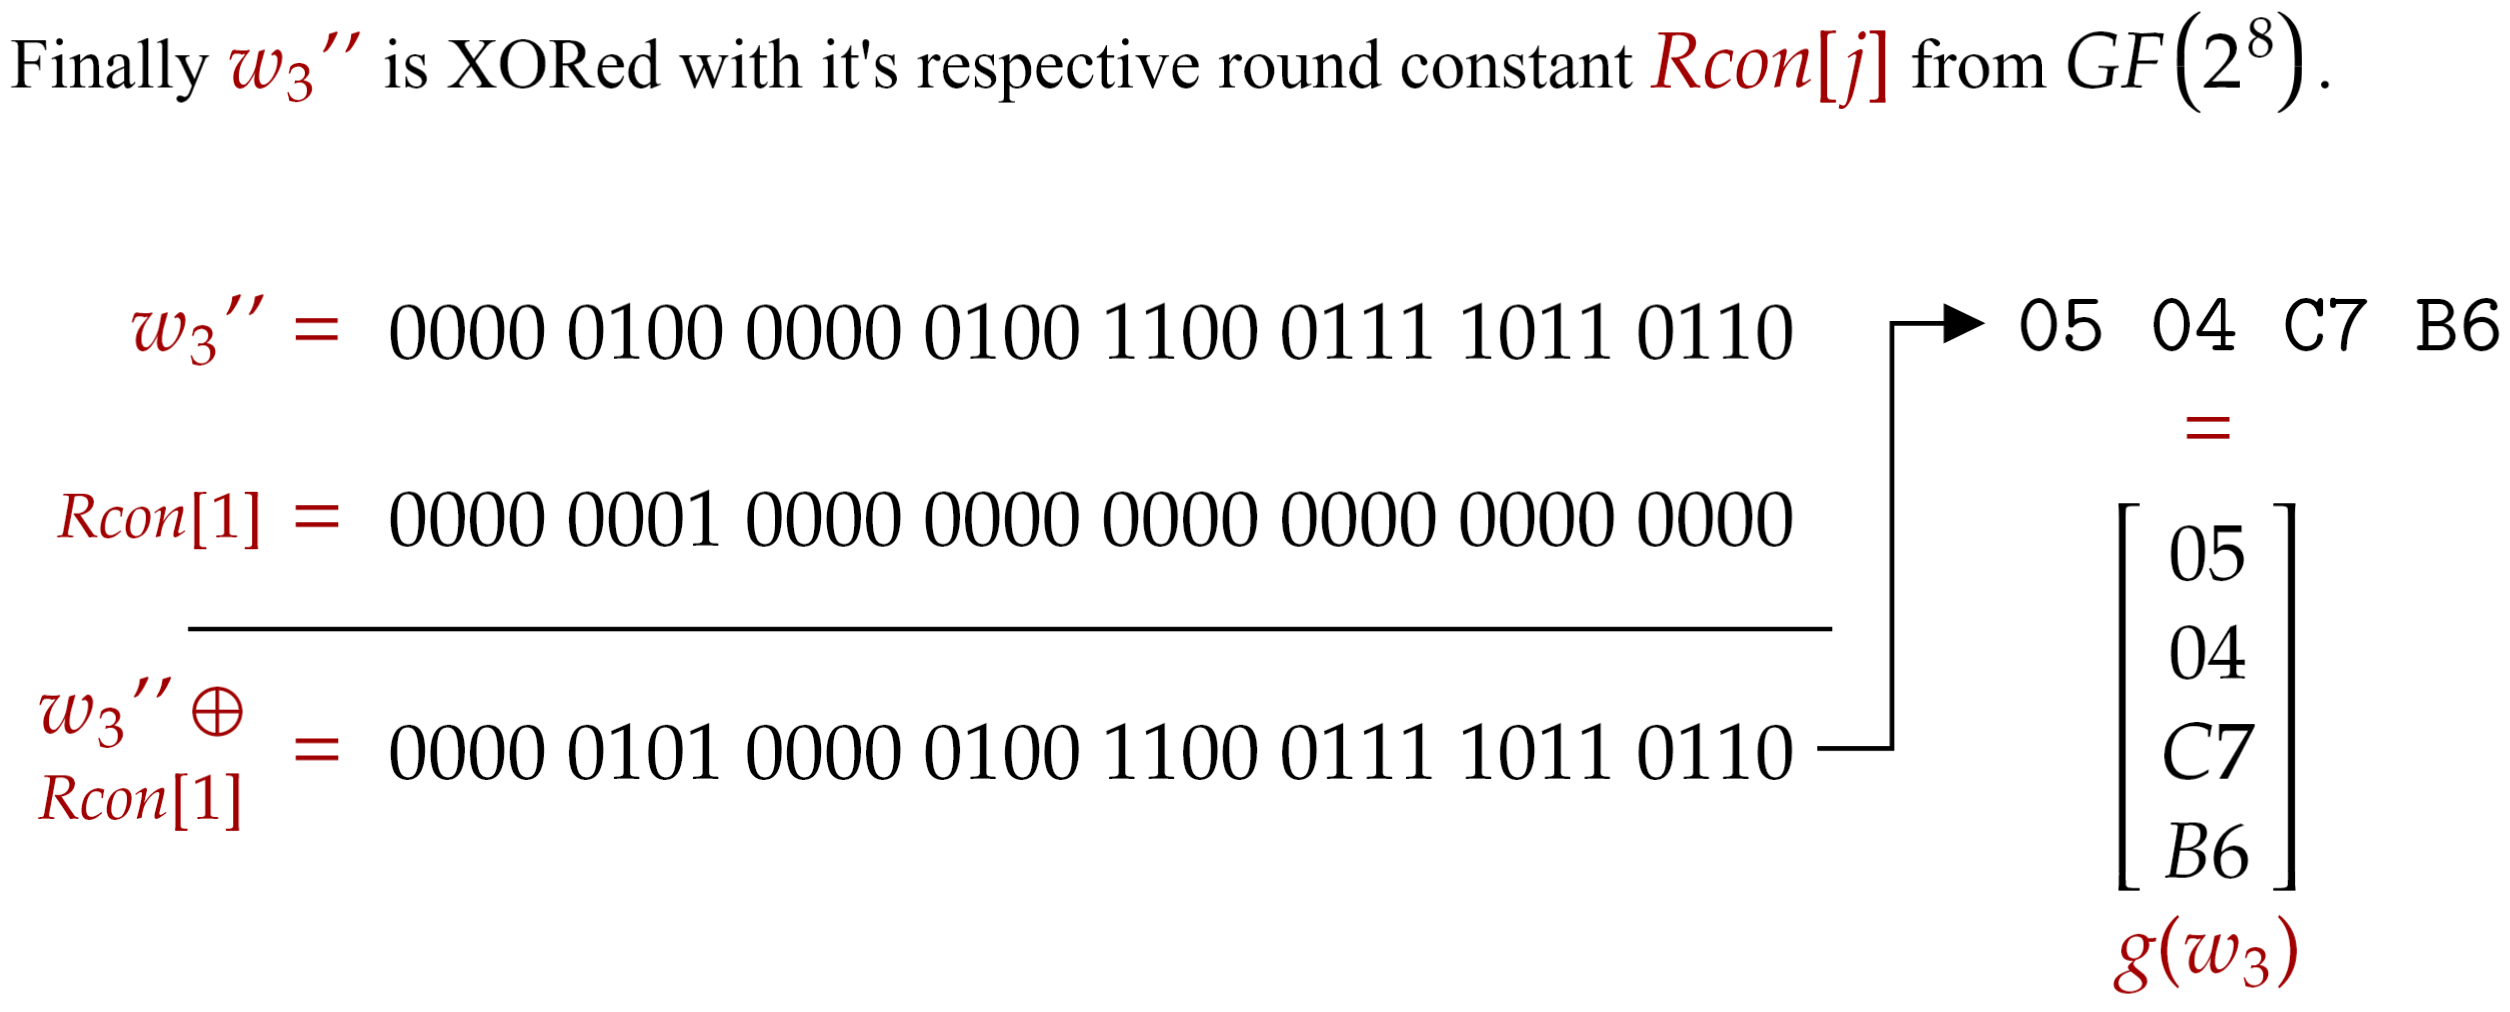
\includegraphics[width=1\textwidth]{Sections/sec/enc/aes/rcon.png}

\newpage 

\noindent
All together:\\

\hspace{-2em}
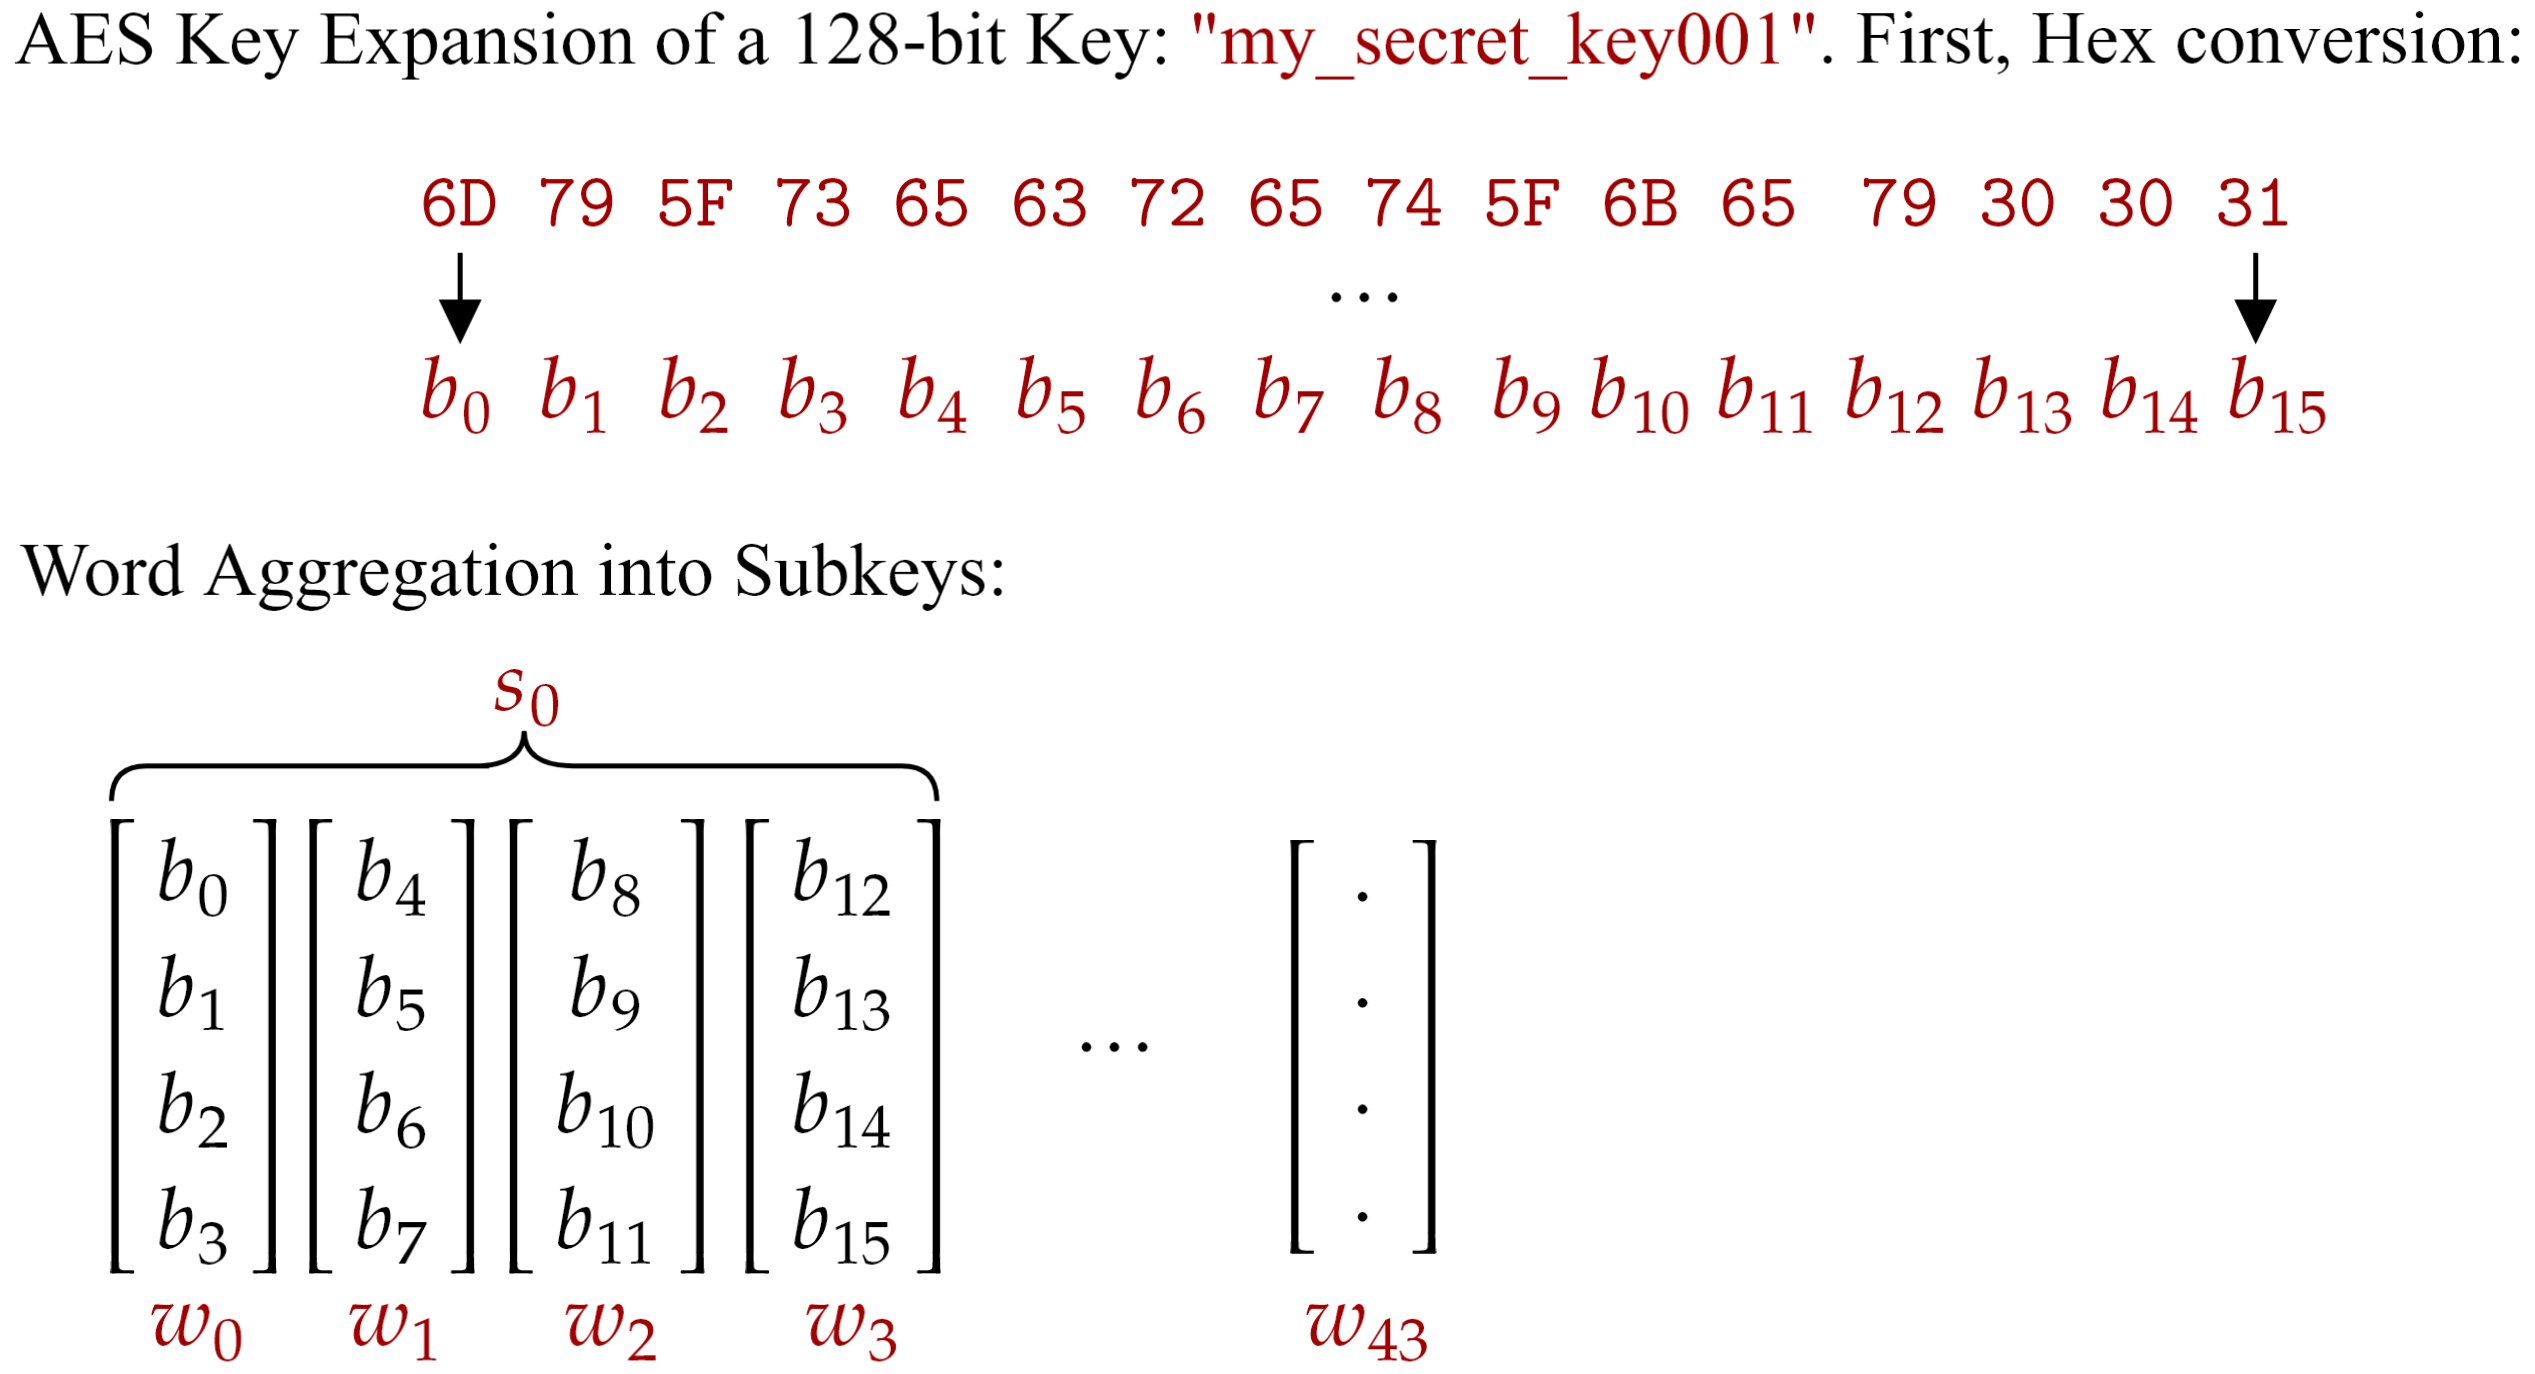
\includegraphics[width=1\textwidth]{Sections/sec/enc/aes/recap1.png}

\hspace{-2em}
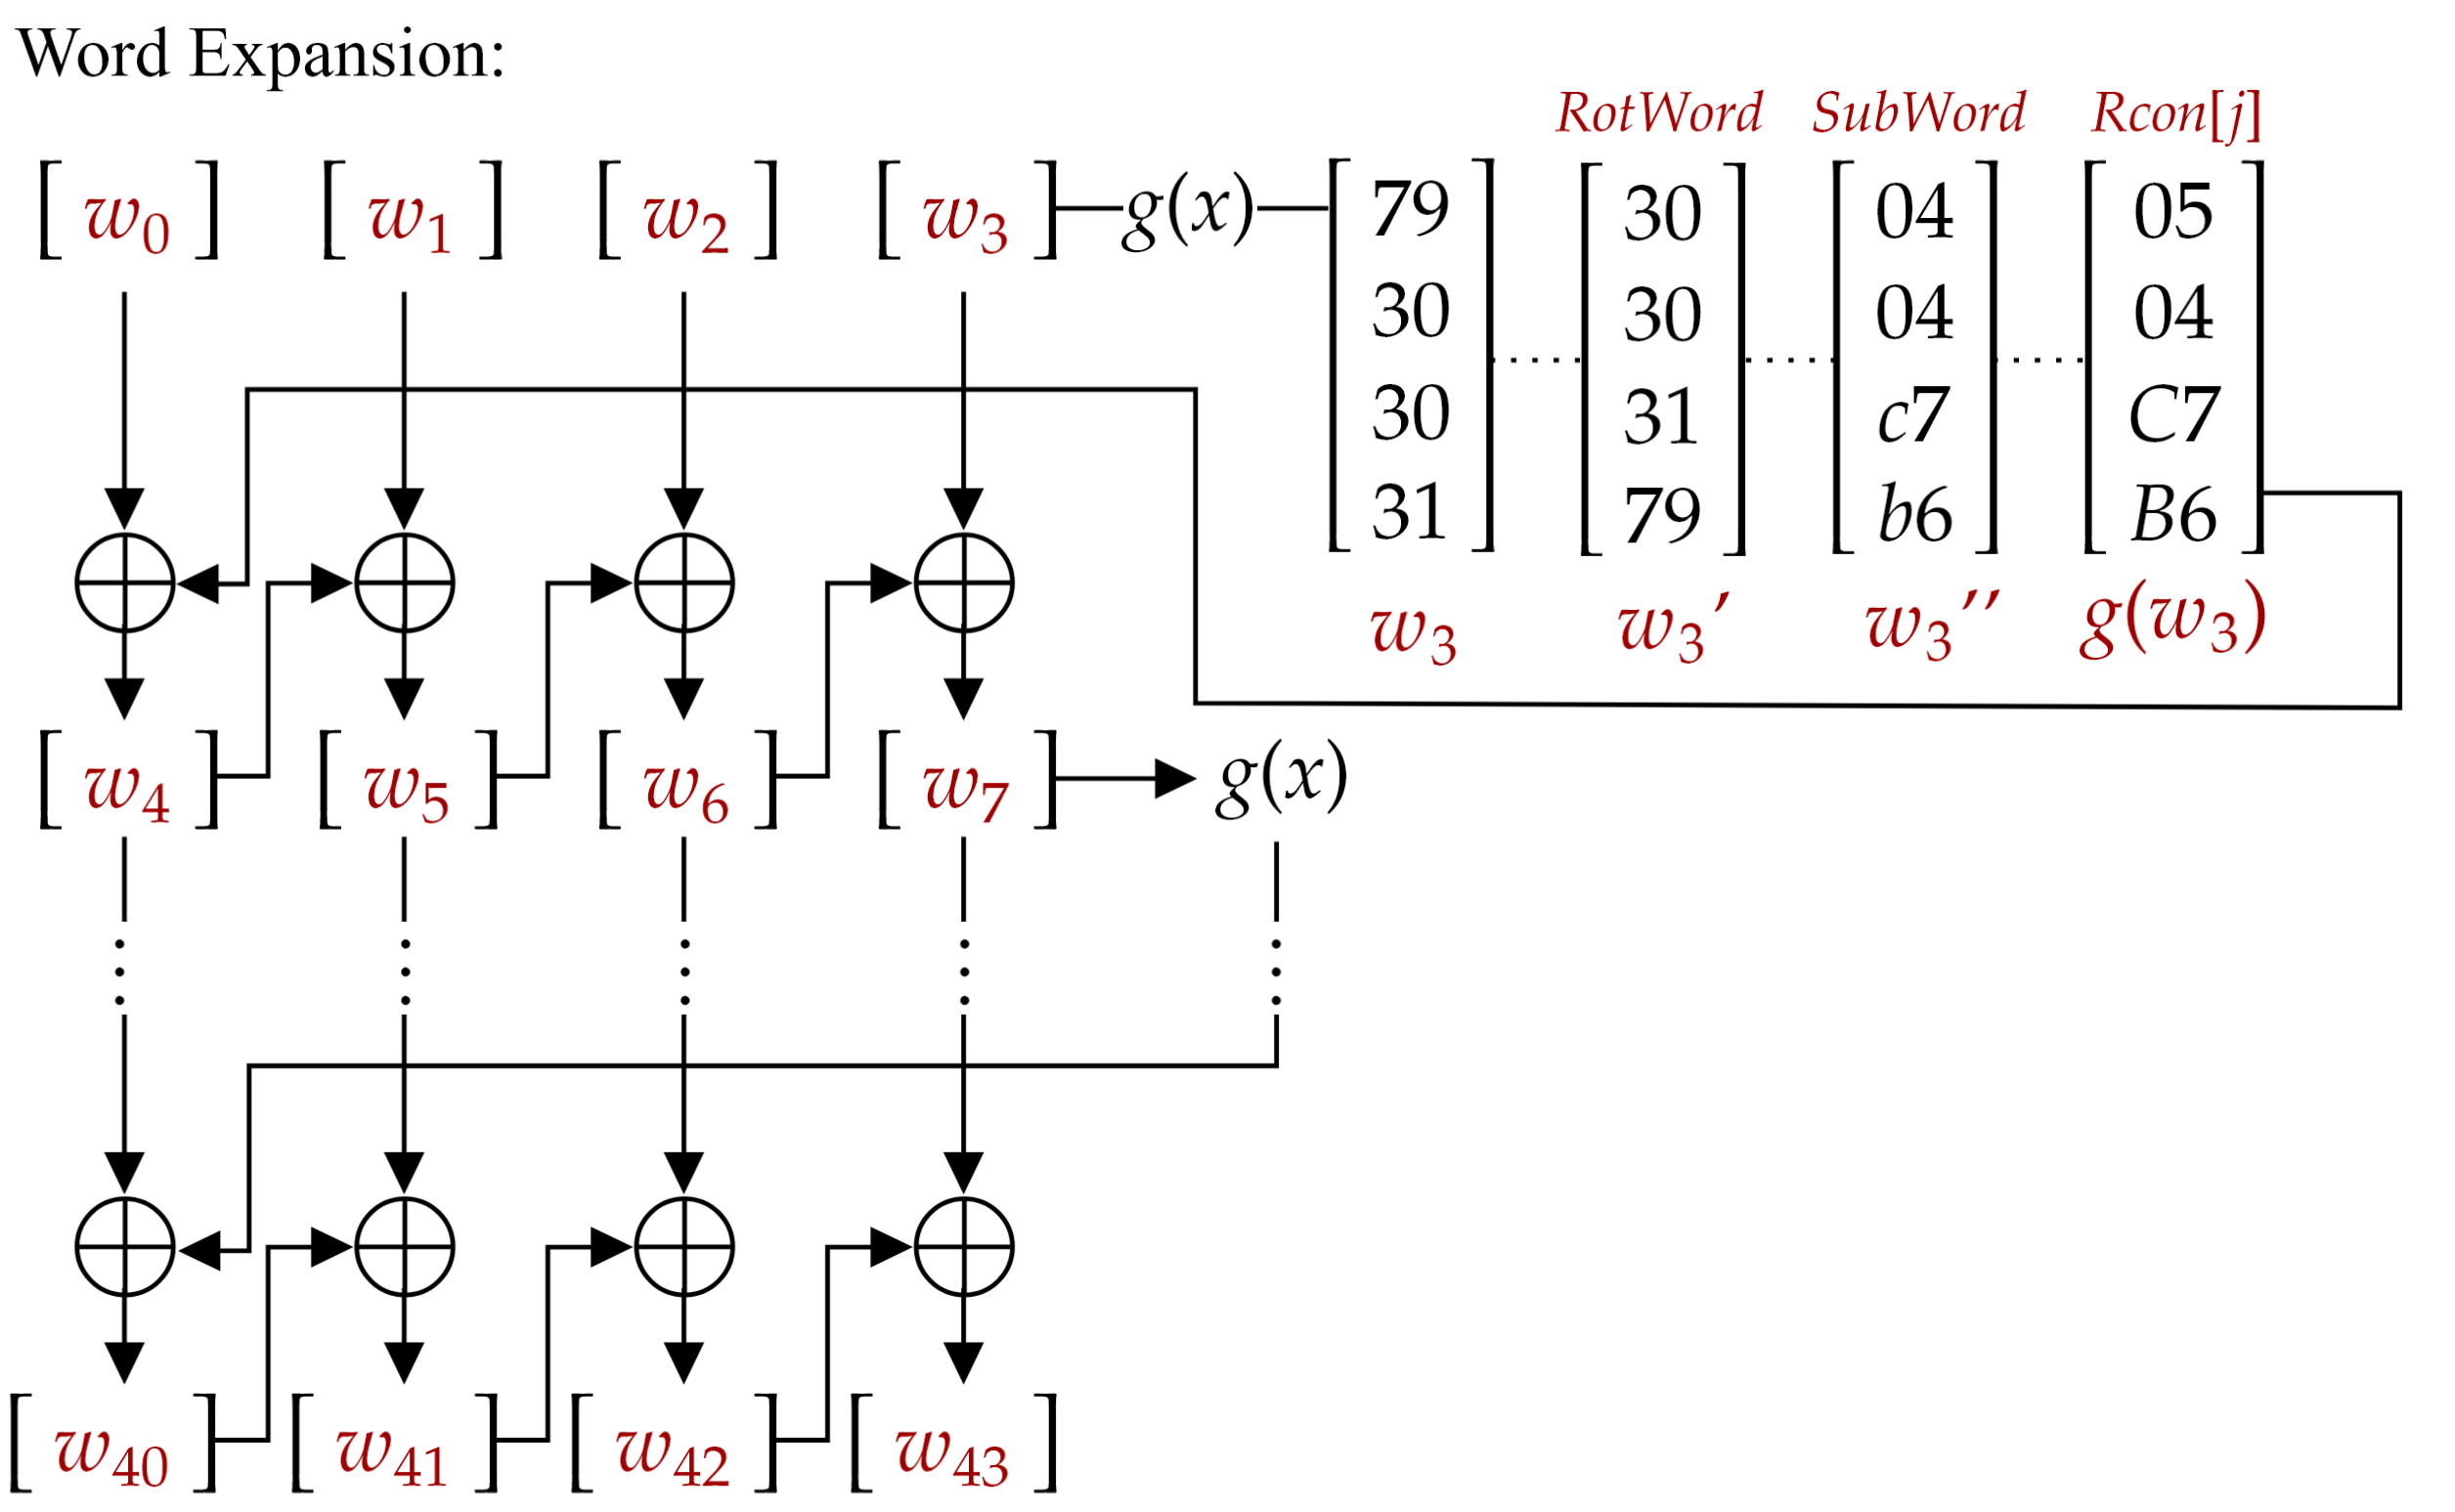
\includegraphics[width=1\textwidth]{Sections/sec/enc/aes/recap2.png}

\vspace{1em}
\noindent
This is AES Key Expansion.

\newpage 

\noindent
Now to discuss the AES encryption process.\\
\vspace{1em}
\hspace{-3em}
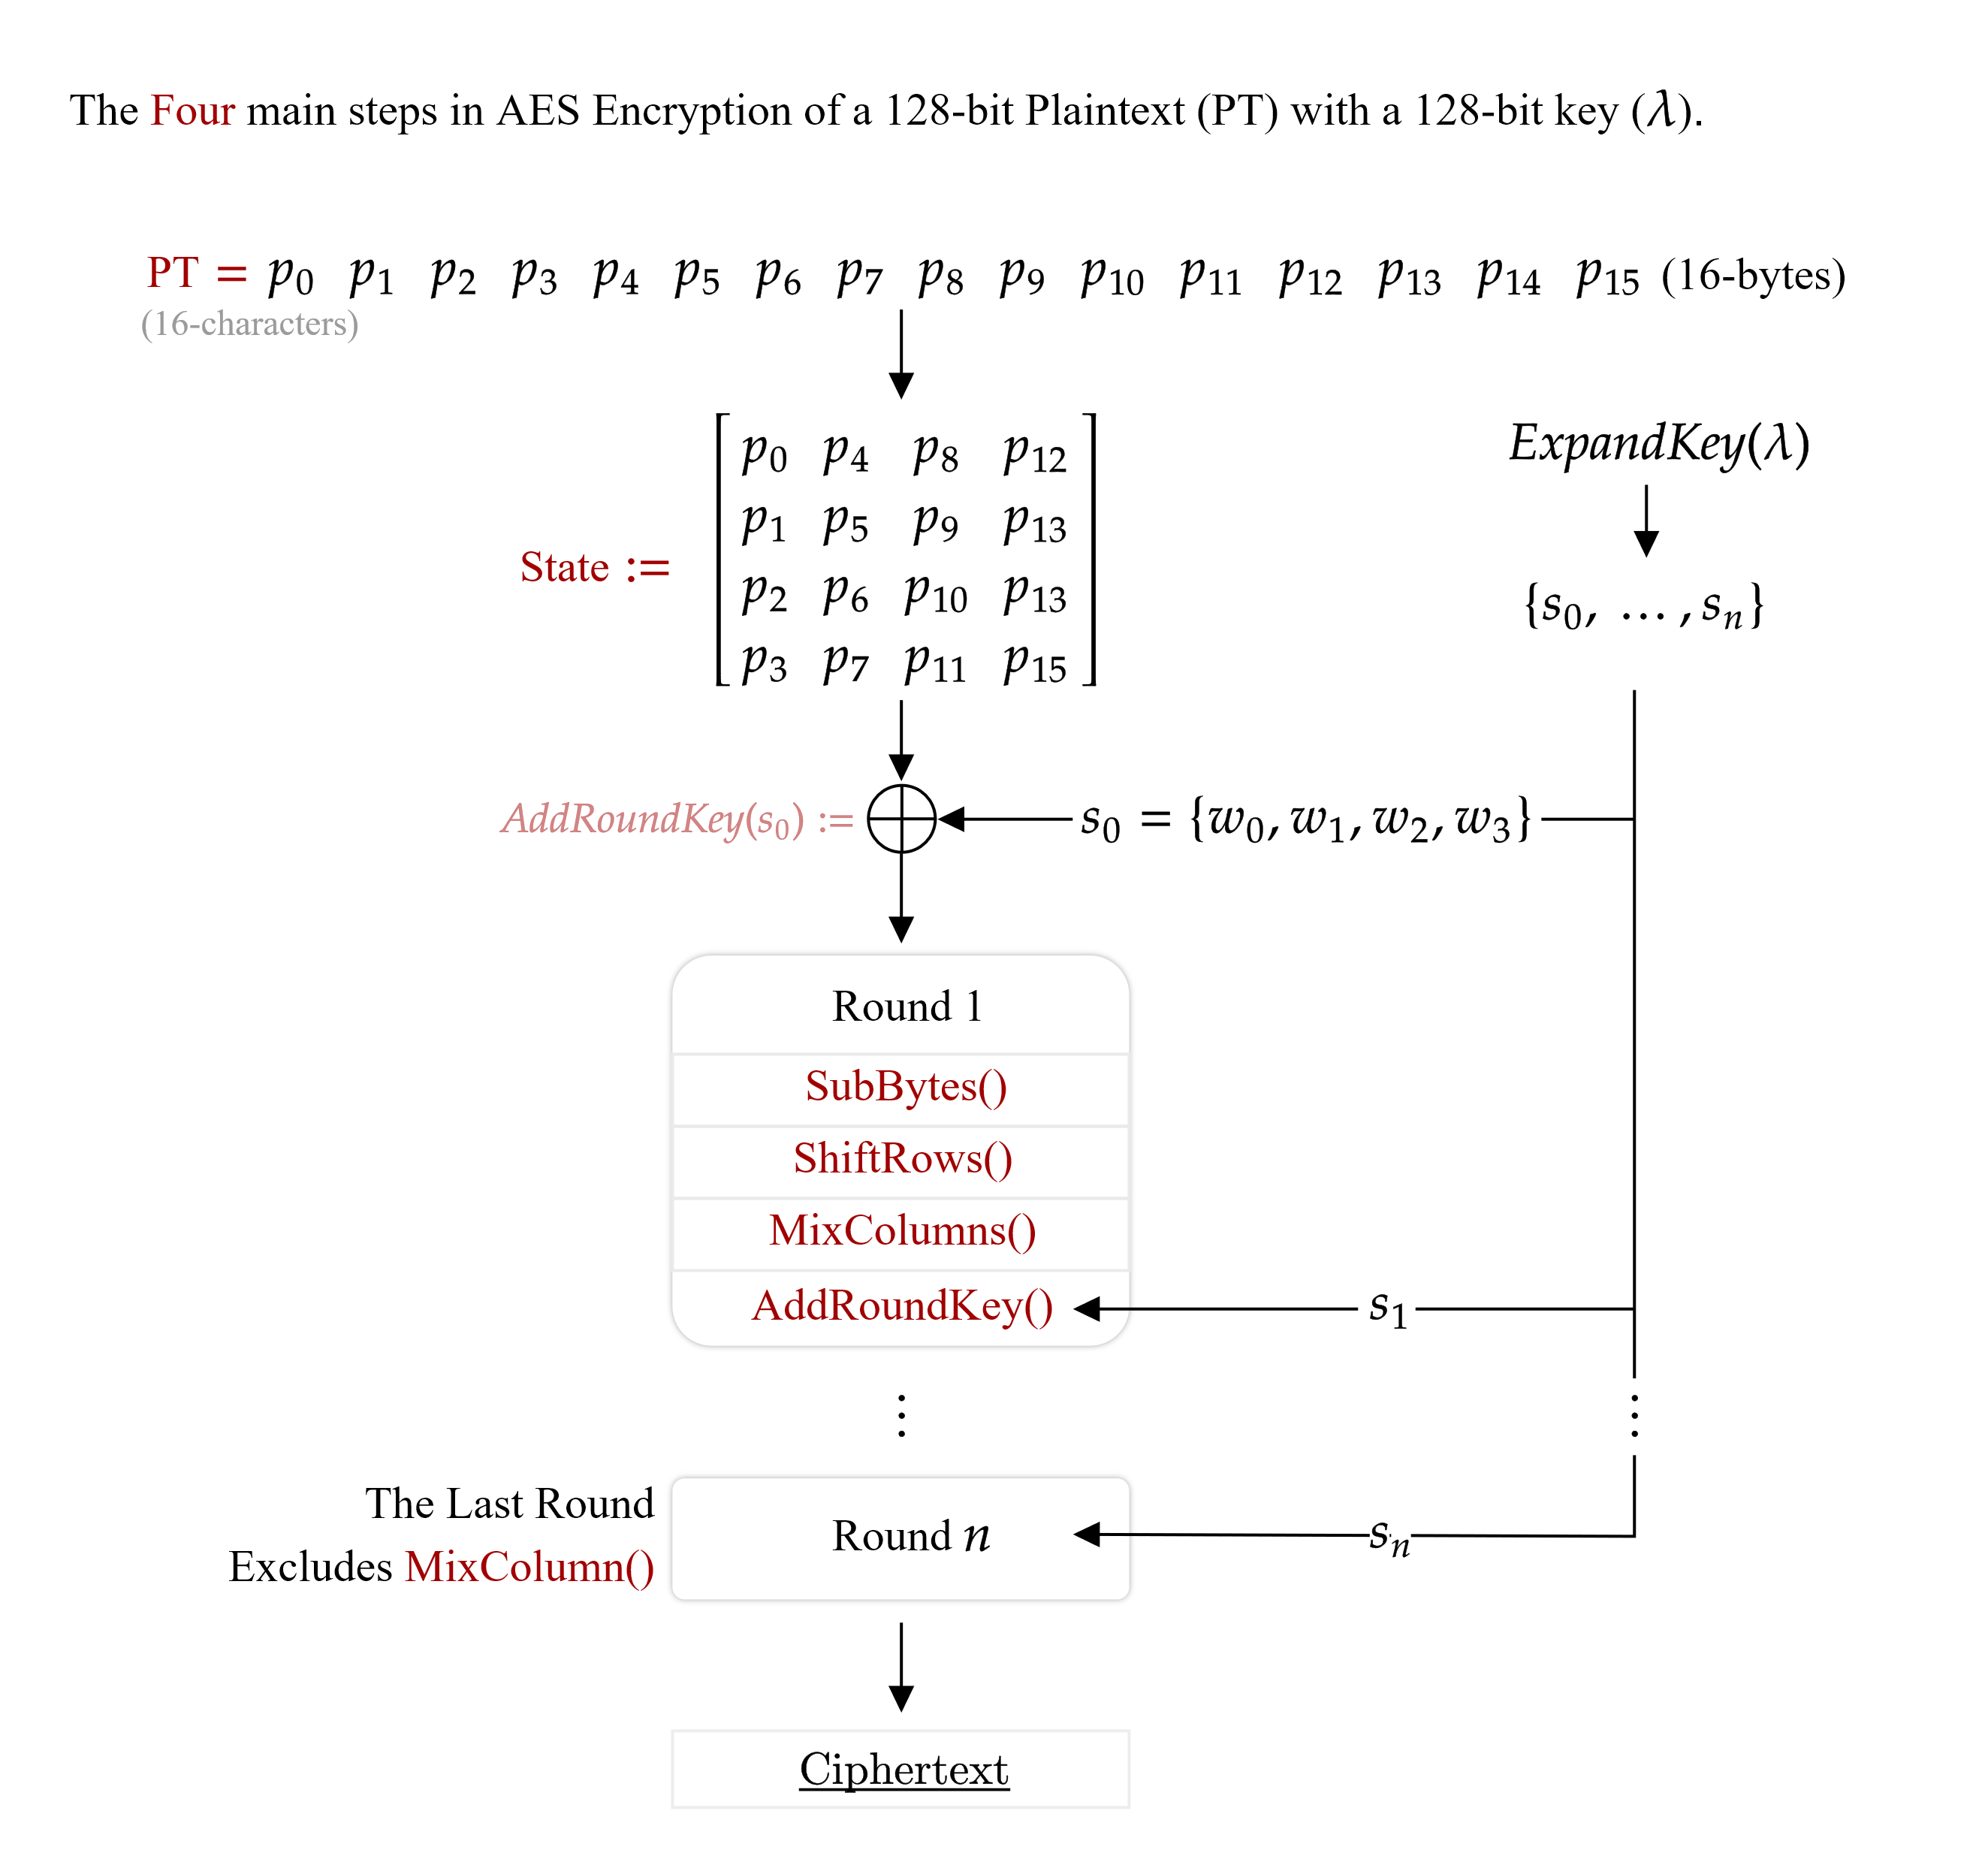
\includegraphics[width=1.1\textwidth]{Sections/sec/enc/aes/trans/high.png}

\vspace{2em}
\noindent
First the PT is transformed into a $4\times4$ matrix, called the \textbf{State}. The initial transformation is the \textbf{AddRoundKey} operation,
which XORs each column of the state with sub-key\\
$s_0=\{w_0,w_1,w_2,w_3\}$. I.e., $[p_0, p_1, p_2, p_3] \oplus [w_0]$ and so on. Recall $w_0=[b_0,b_1,b_2,b_3]$ 
for some byte $b_i$ of the initial key.
\newpage 

\noindent
To elaborate on the AddRoundKey operation:\\

\hspace{-3em}
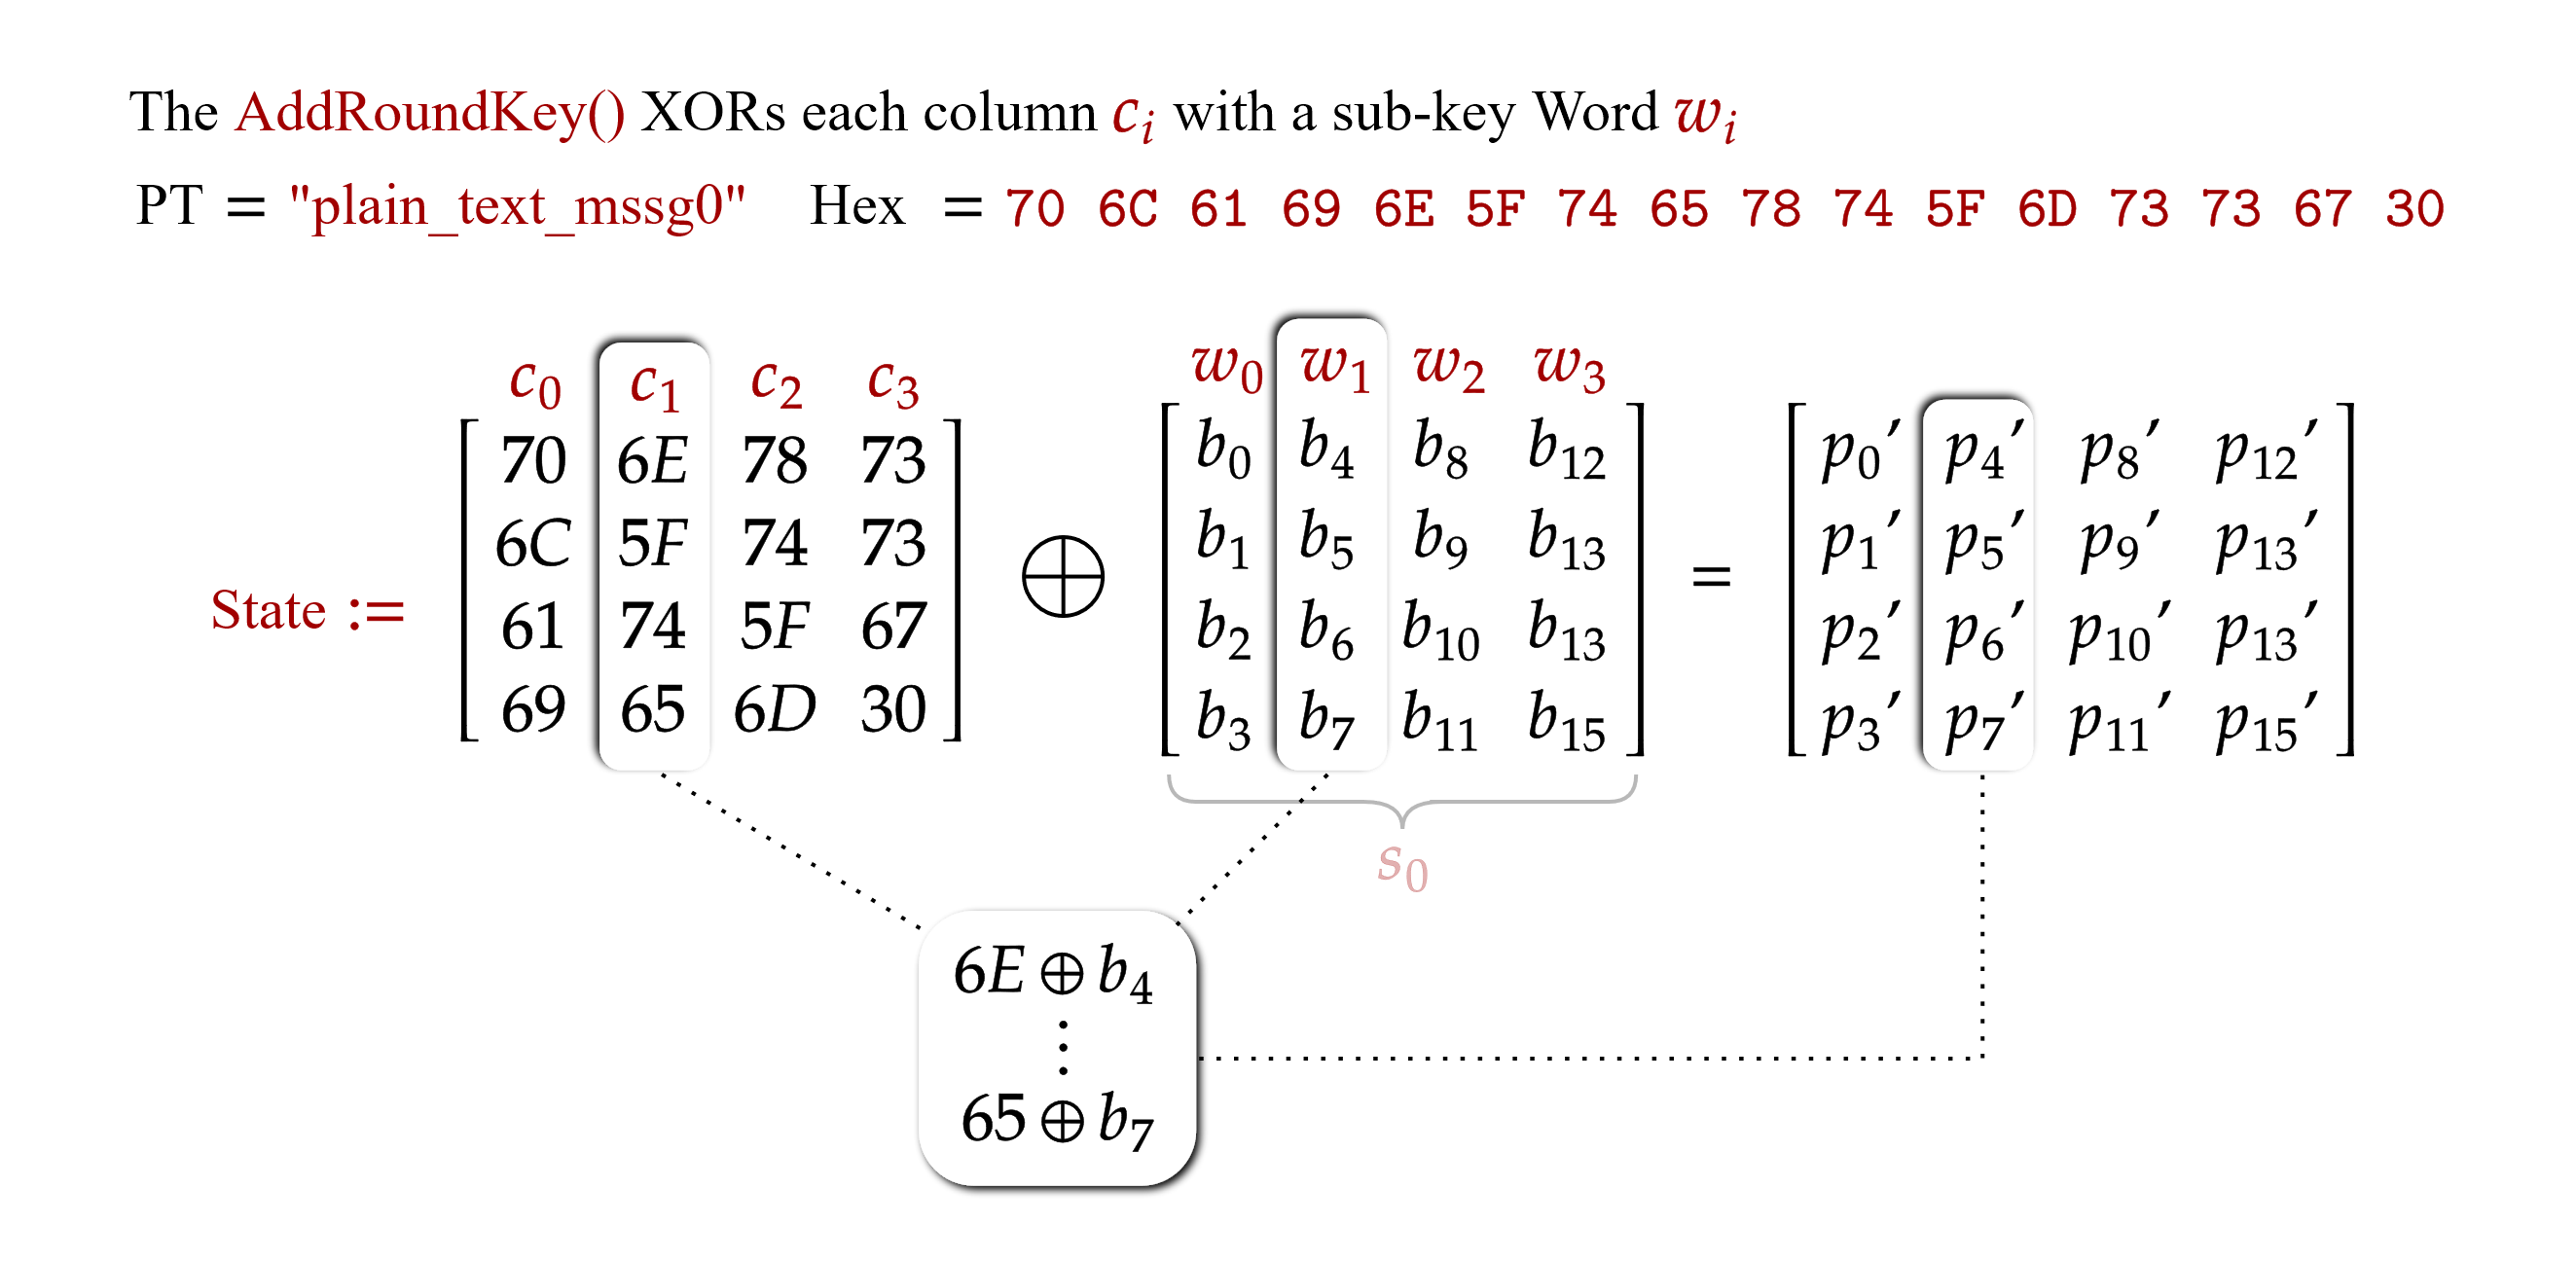
\includegraphics[width=1.1\textwidth]{Sections/sec/enc/aes/trans/add.png}
AddRoundKey takes a sub-key $s_i$ and XORs each Word $w_i$ with the corresponding column $c_i$ of the State.
\vspace{5em}

\hspace{-3em}
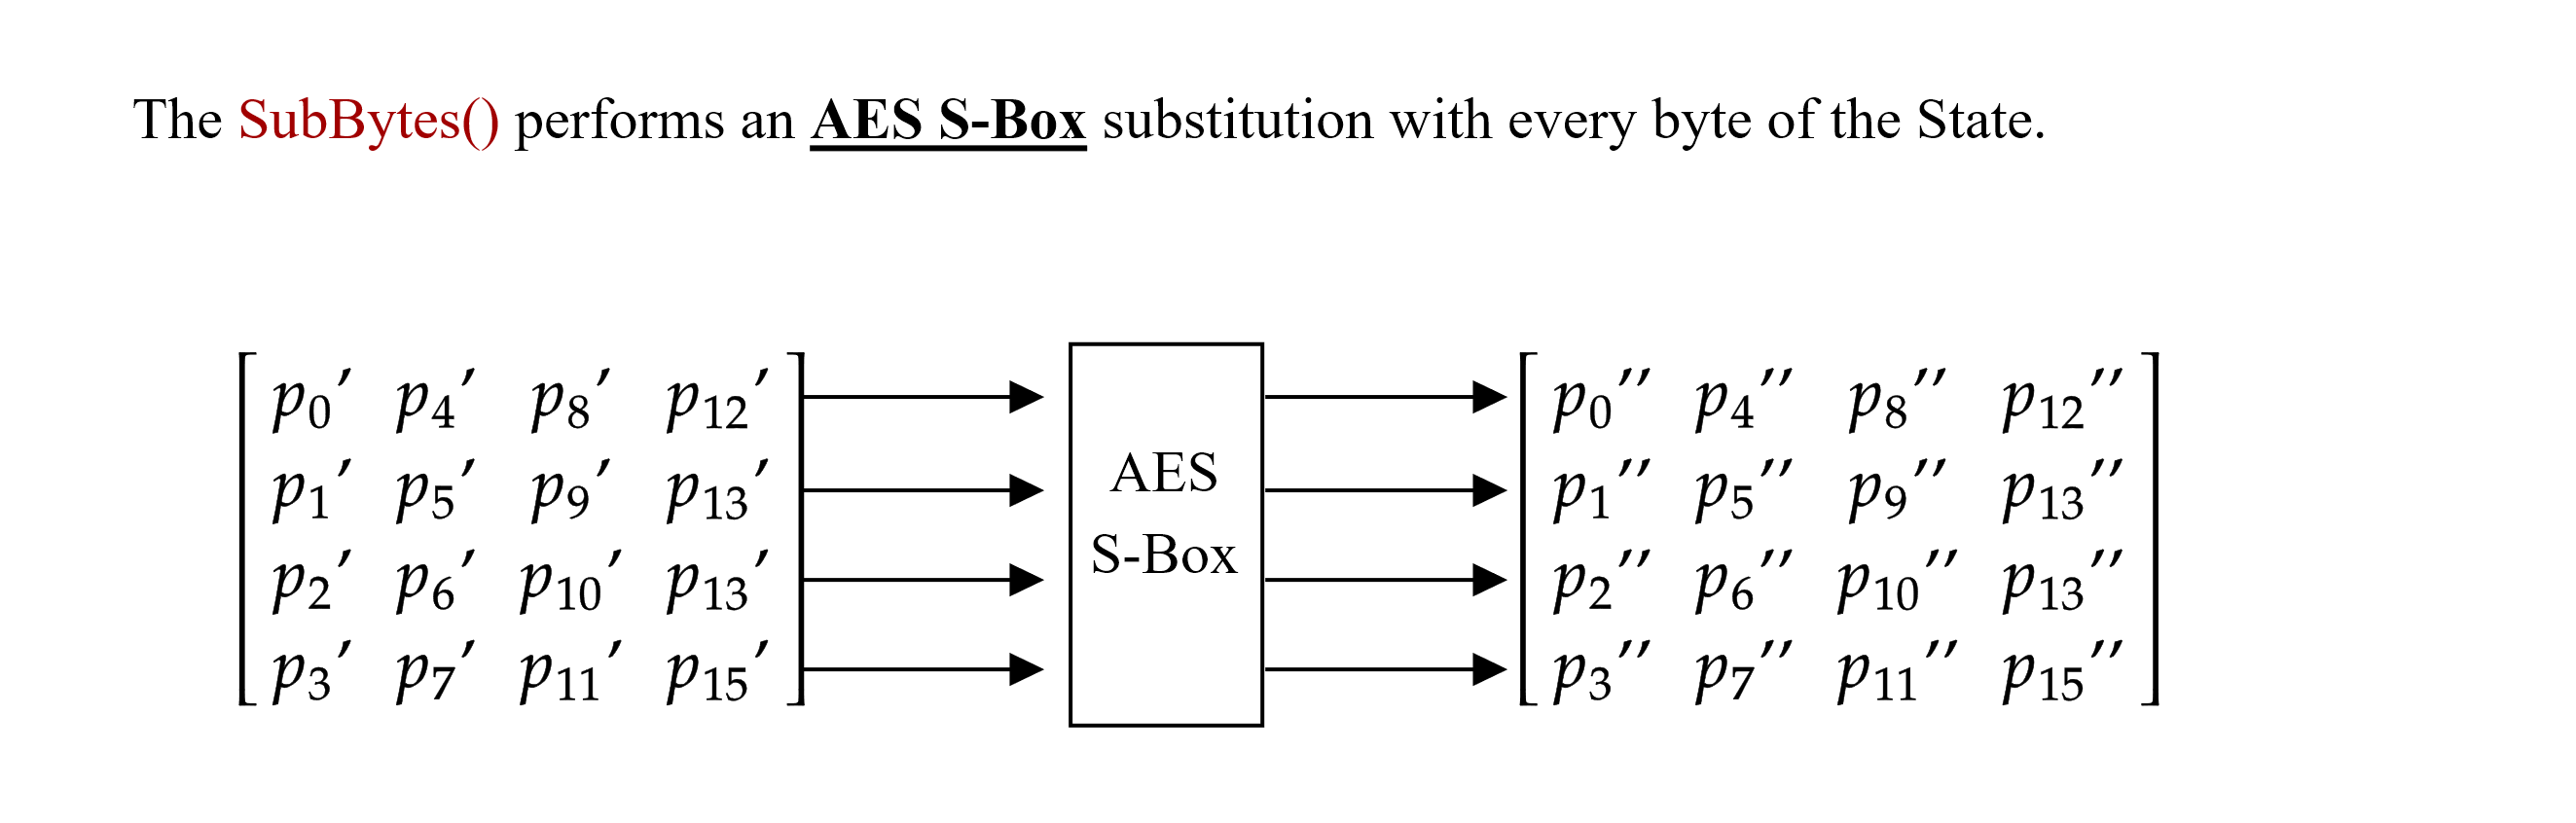
\includegraphics[width=1.1\textwidth]{Sections/sec/enc/aes/trans/sub.png}

\noindent
Just like in Key Expansion's (\ref{theo:key_expansion}) use of the S-Box on the last word of each sub-key. The PT undergoes 
a full substitution with the S-Box.

\newpage 

\hspace{-3em}
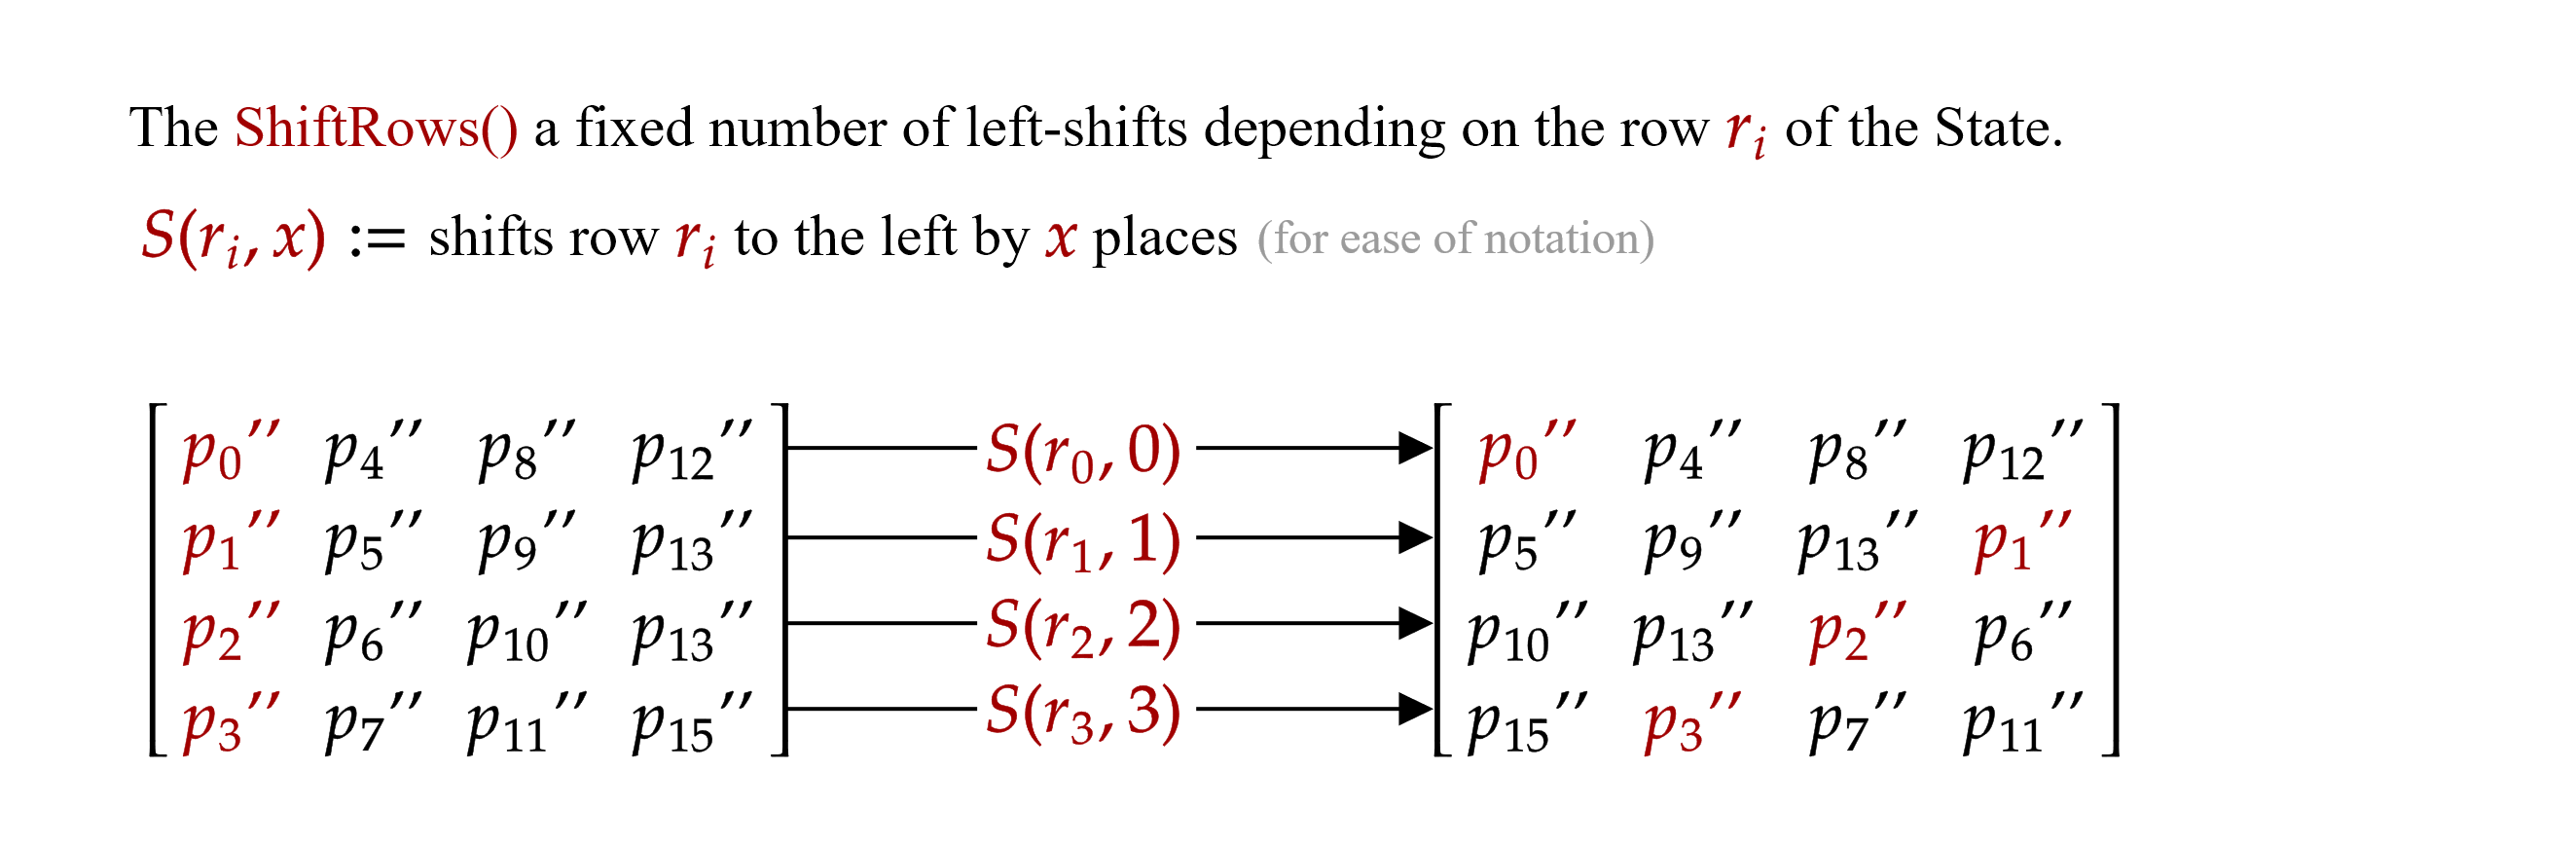
\includegraphics[width=1.1\textwidth]{Sections/sec/enc/aes/trans/shift.png}
\vspace{-1em}


\noindent
\underline{Below, the notation $\{01\}$ refers to a hex value.}\\

\vspace{-1em}
\hspace{-3em}
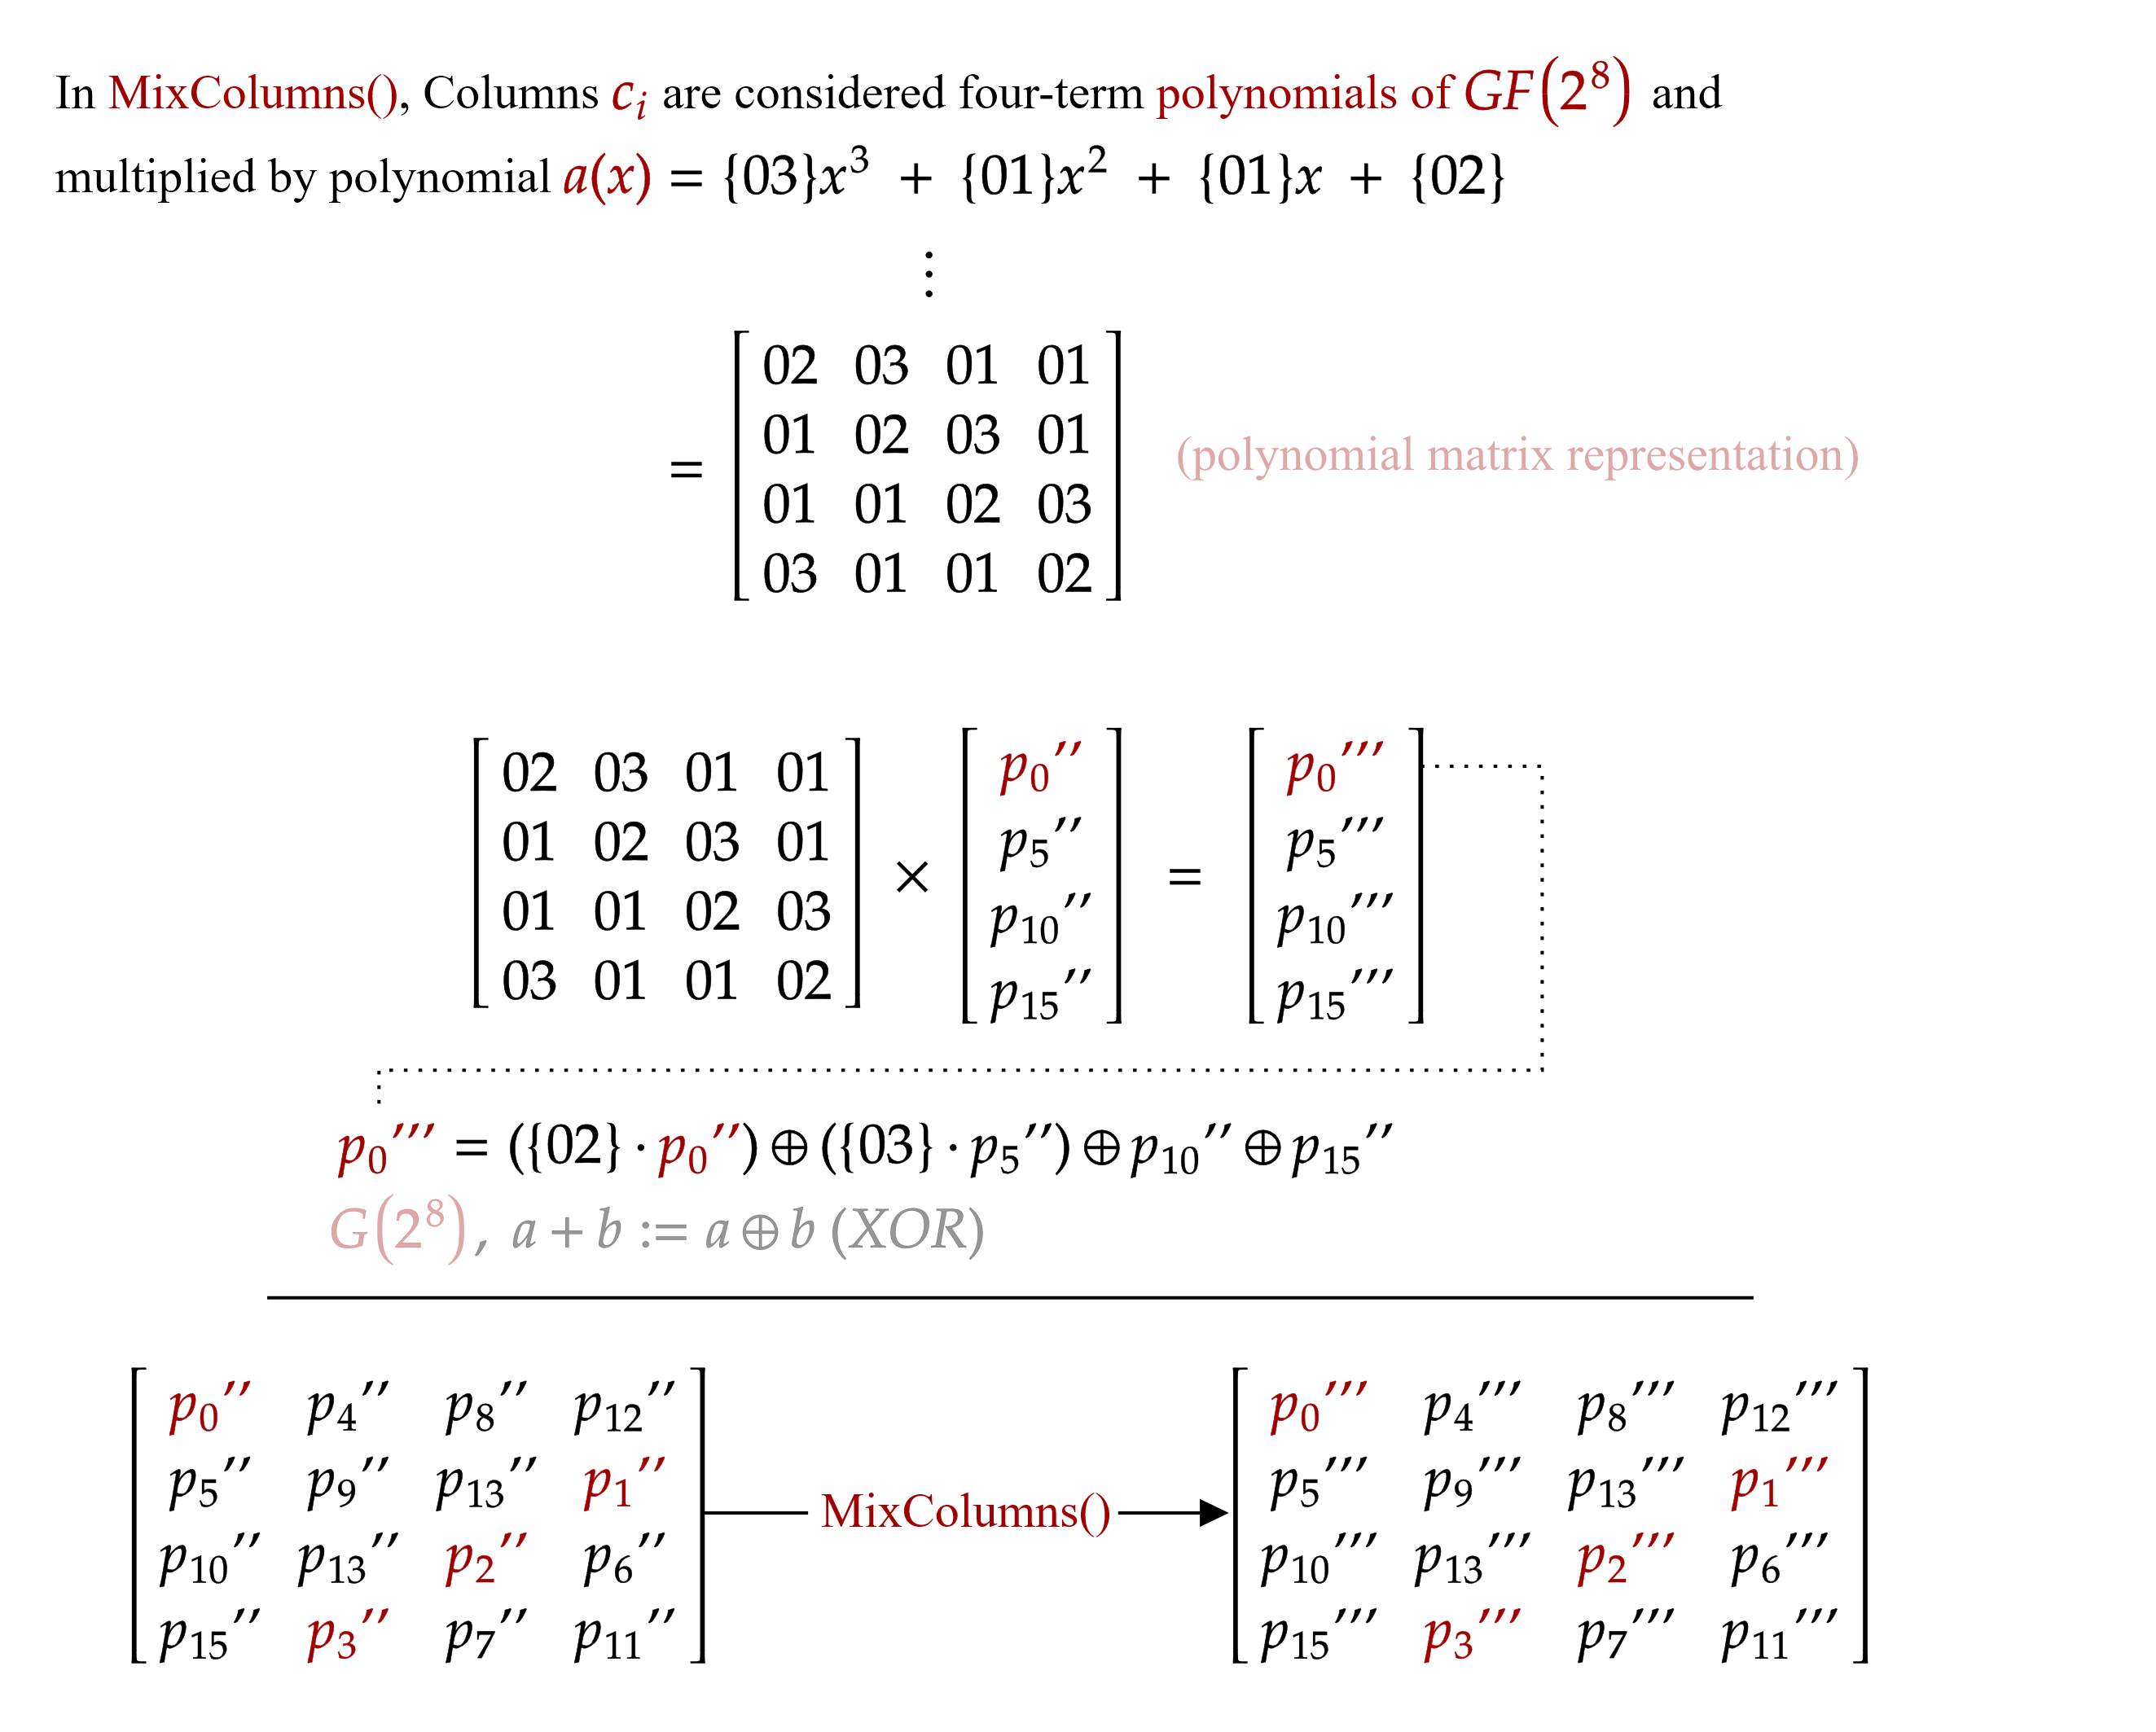
\includegraphics[width=1.1\textwidth]{Sections/sec/enc/aes/trans/mix.png}

\newpage

\noindent
This is the AES Encryption \& Decryption.

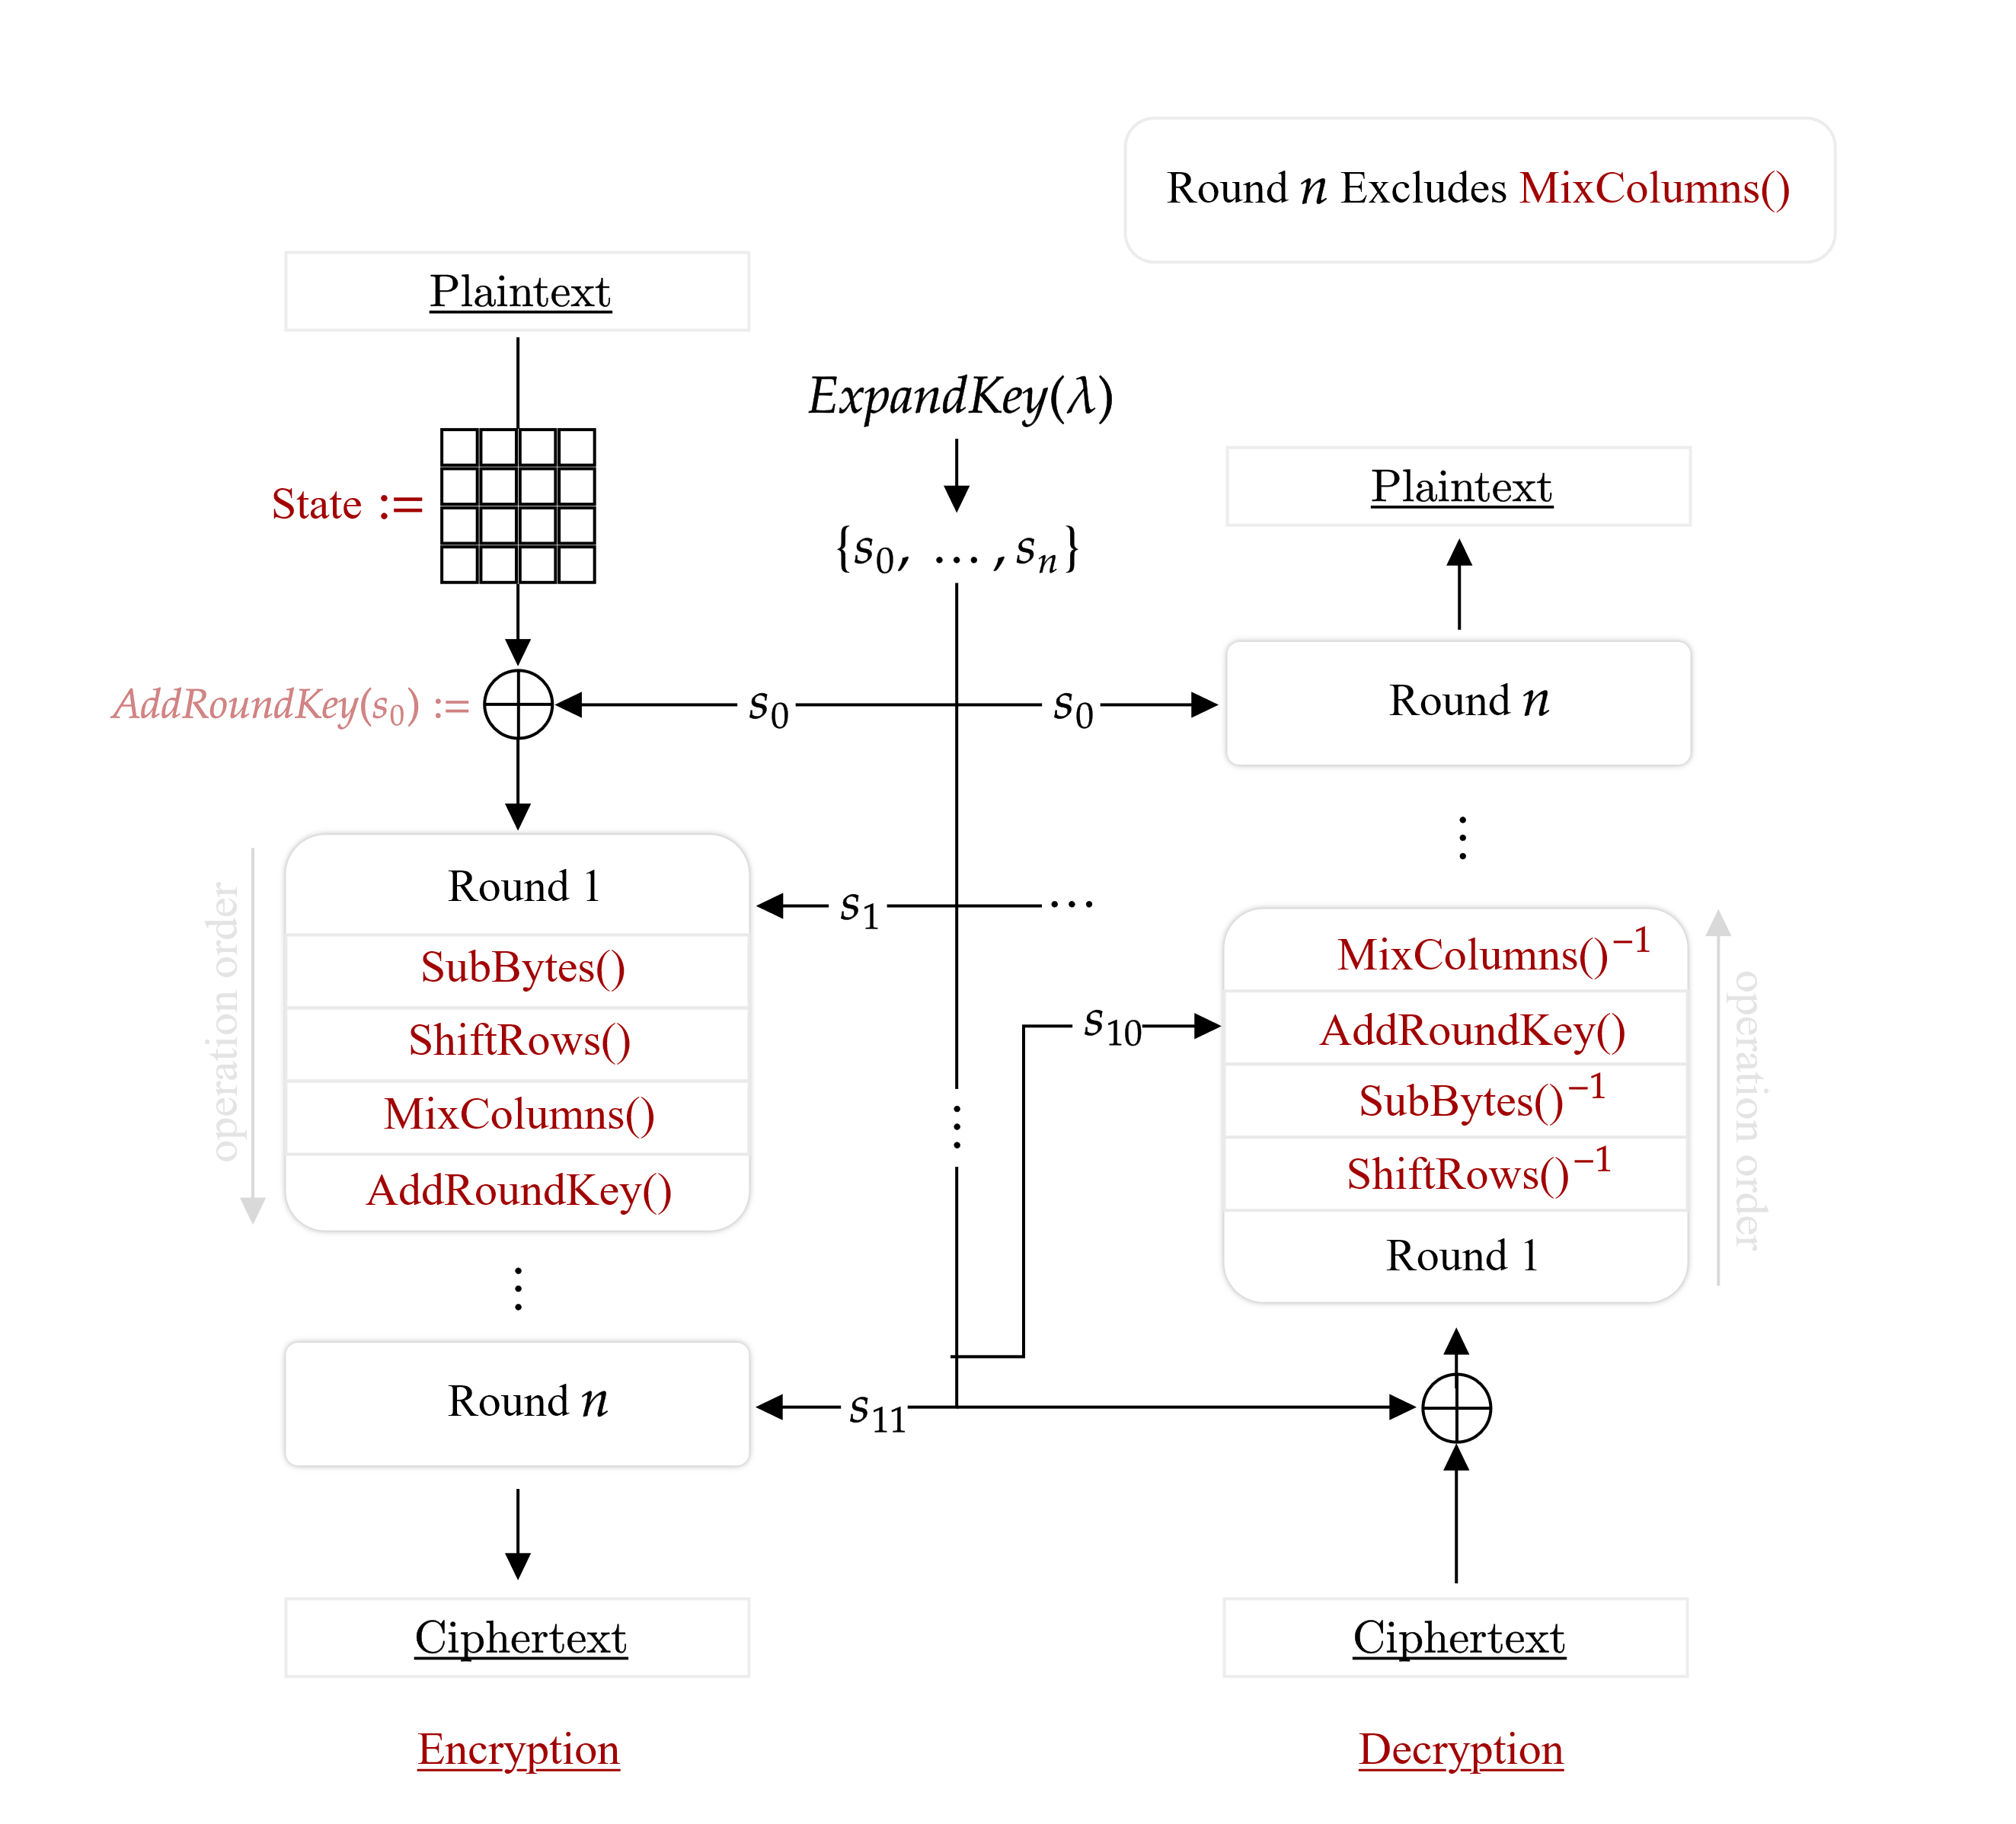
\includegraphics[width=1.1\textwidth]{Sections/sec/enc/aes/trans/ende.png}

\vspace{1em}
\noindent
For Decryption, the last scheduled key for Encryption is used as the initial transformation. Note the inverse 
operations of Decryption follow a different order than Encryption, and use 
their respective inverse functions. This covers the basics of AES.
